\documentclass[lettersize,journal]{IEEEtran}
\usepackage{amsmath,amsfonts}
\usepackage{algorithmic}
\usepackage{algorithm}
\usepackage{array}
\usepackage[caption=false,font=normalsize,labelfont=sf,textfont=sf]{subfig}
\usepackage{textcomp}
\usepackage{stfloats}
\usepackage{url}
\usepackage{verbatim}
\usepackage{graphicx}
\usepackage{cite}

% added packages from authors
\usepackage{xcolor}
\usepackage{booktabs} % for \midrule in tables
\usepackage{hhline}
\usepackage{bbm}
\usepackage{bm}
\usepackage{makecell}

\hyphenation{op-tical net-works semi-conduc-tor IEEE-Xplore}
% updated with editorial comments 8/9/2021

\begin{document}

\title{Load shifting versus manual frequency reserve: \\ Which one is more appealing to flexible loads?}

\author{Peter A.V. Gade\textsuperscript{*}\textsuperscript{\textdagger}, Trygve Skjøtskift\textsuperscript{\textdagger}, Henrik W. Bindner\textsuperscript{*}, Jalal Kazempour\textsuperscript{*} \\
    \textsuperscript{*}Department of Wind and Energy Systems, Technical University of Denmark, Kgs. Lyngby, Denmark \\
    \textsuperscript{\textdagger}IBM Client Innovation Center, Copenhagen, Denmark
    % <-this % stops a space
    \thanks{Corresponding author. Tel.: +45 24263865. \\ Email addresses: pega@dtu.dk (P.A.V. Gade), Trygve.Skjotskift@ibm.com (T. Skjøtskift), hwbi@dtu.dk (H.W. Bindner), jalal@dtu.dk (J. Kazempour).}% <-this % stops a space
    \thanks{Manuscript received April 19, 2021; revised August 16, 2021.}}

% \footnote{Corresponding author. Tel.: +45 24263865. \\ Email addresses: pega@dtu.dk (P.A.V. Gade), Trygve.Skjotskift@ibm.com (T. Skjøtskift), hwbi@dtu.dk (H.W. Bindner), jalal@dtu.dk (J. Kazempour).}

% The paper headers
\markboth{Journal of \LaTeX\ Class Files,~Vol.~14, No.~8, August~2021}%
{Shell \MakeLowercase{\textit{et al.}}: A Sample Article Using IEEEtran.cls for IEEE Journals}

\IEEEpubid{0000--0000/00\$00.00~\copyright~2021 IEEE}
% Remember, if you use this you must call \IEEEpubidadjcol in the second
% column for its text to clear the IEEEpubid mark.

\maketitle

% \tableofcontents

\begin{abstract}
    % \section*{Abstract}

This paper investigates how a flexible load can deliver flexibility for manual frequency reserves and load shifting. We discuss the advantages and disadvantages of the two and their appeal from a monetary point of view. To this end, a grey-box model of a supermarket freezer is created to describe its temperature dynamics using real data from a supermarket in Denmark. A two-stage stochastic mixed-integer linear program (MILP) maximizes the flexibility value from the freezer where two solution strategies for manual frequency reserves are presented. Load shifting shows to be more profitable than manual frequency reserves on unseen price data, but is also more consequential for the temperature in the freezer than flexibility provision for manual frequency reserves.

\end{abstract}

\begin{IEEEkeywords}
    Demand-side flexibility.
\end{IEEEkeywords}

\section{Introduction}

Power consumers are looking to reduce costs by any means due to sky-rocketing energy- and gas prices. In Denmark, supermarkets are especially exposed due to their high energy consumption, and they are actively looking into initiatives to reduce their electricity bill. One of these initiatives is the application of demand-side flexibility, whereby a supermarket can shift consumption in time when spot prices are lower or when the power grid needs up-regulation. There are thousands of supermarkets in Denmark willing to provide flexibility, and their freezers are especially suited for this as they constitute a big share of their energy consumption.

IBM is currently developing a software platform - called Flex Platform - that can harness flexibility from industrial and commercial consumers for bidding in ancillary service markets by a balance responsible party (BRP). One large supermarket chain in Denmark has already signed up for the Flex Platform, and another supermarket chain is currently exploring the possibility of joining.

However, the monetary benefit still remains uncertain. In this paper, we describe how to utilize a supermarket freezer's flexibility with respect to manual frequency restoration reserves (mFRR)\footnote{The term will be used for the remainder of the paper and is equivalent to tertiary reserves.} and load shifting, and thereby the incentives for doing so.

To this end, many studies have used grey-box models to capture the most fundamental physics while using data to calibrate the model. A grey-box model can illustrate the concept of flexibility well, and we show how it can be used for simulations. Such a model can also readily be used in a mathematical optimization framework to, e.g., reduce costs or maximize earnings from flexibility. An optimization model can be used to obtain a simple policy for how to shift consumption in time and how to provide flexibility for mFRR.

In this work, we determine the monetary benefit of flexibility using such an optimization model with two solution strategies: 1) one using a five days lookback on prices and 2) one using 2021 data for prices. We evaluate the model on out-of-sample 2022 price data.

Our contribution is two-fold: 1) we show how to model mFRR reservation, bidding, and activation using a novel two-stage stochastic program and 2) we investigate and discuss the incentives to utilize demand-side flexibility for mFRR versus load shifting which is interesting from both a power system- and consumer perspective. % For example, if the consumers are incentivized to load shift instead of providing mFRR, the power system will not necessarily benefit, consumers will only benefit in the short-term.

\IEEEpubidadjcol


\subsection{Dilemma: mFRR vs load shifting}

For consumers that are actively looking to reduce costs, it is important to understand the monetary benefit of flexibility. From their perspective, it is natural to first look into load shifting at first, since it is the most obvious and easy way to utilize flexibility. Here, load shifting simply refers to shifting consumption to another point in time, typically when spot prices are lower.

However, load shifting is not necessarily helping the power grid.
In fact, if a significant amount of consumers started to do it, it could be detrimental to the power grid by moving peak consumption to a different time of the day.
%In fact, if a significant amount of consumers move a large part of their consumption to a different time of the day, that could be detrimental to the power grid by creating new and even more pronounced peaks.
Intriguingly, many industrial and residential consumers have already started shifting demand to some degree, as a response to the energy crisis.
As a result, load shifting might provide \textit{short-term} monetary benefit, but it is not necessarily helping the power grid in the long run.

%Instead, consumers could opt for offering ancillary services, for which they are paid for providing flexibility through an \textit{aggregator}.
Instead, consumers could choose to provide flexibility by offering ancillary services through an \textit{aggregator}, for which they would be compensated.
One such service is mFRR in Denmark, which is a slow-responding reserve used to stabilize frequency in the power grid after fast frequency reserves are depleted. The market for mFRR is usually operated by each country's respective TSO.\footnote{In Denmark, the TSO is Energinet.} mFRR resembles load shifting in the sense that it is the largest energy reserve operated by the TSO, and can be provided by consumers by shifting their consumption in time.\footnote{Likewise, generators provide mFRR by increasing their power generation.}

In order for a freezer to deliver mFRR, it must be part of a bigger portfolio with potentially many small assets to meet the minimum requirements for entering the mFRR market. Furthermore, there might be additional synergy effects such as increased operational flexibility in the control response, rebound, and temperature deviations \cite{koch2011modeling}. However, in this paper it is assumed for simplicity that one freezer delivering mFRR can be scaled to many freezers in the same way (and likewise for load shifting).

Demand response for consumers participating in mFRR versus load shifting will therefore look similar. From the consumers' perspective, it is of great interest to investigate the monetary benefit of participating in each, and it is important to understand the incentive of consumers to participate in mFRR from a TSO perspective as well.

\subsection{Research questions}

To understand the incentives to participate in load shifting and mFRR from a flexible consumer's perspective, this work aim to investigate and answer the following research questions:

\begin{itemize}
    \item How can a supermarket freezer's flexibility be characterized?
    \item How much monetary benefit can a freezer provide for mFRR?
    \item How much monetary benefit can a freezer provide for load shifting?
    \item What are the advantages and disadvantages of participating in mFRR versus load shifting?
\end{itemize}

Some of these questions have been looked at extensively in literature, so we first provide a brief literature review to pinpoint where new work is required and how our work relates to existing work.

\subsection{Literature review}

Demand-side flexibility has been extensively studied. The approach taken in each study is very much dependent on the perspective from which flexibility is utilized. Often, full knowledge and control of all assets is assumed. An often overlooked implicit assumption is that the aggregator and/or trading entity are the same, with an exclusive business relationship to flexible consumers \cite{gade2022ecosystem}. The incentives and investments required for delivering flexibility for the flexible consumer are often overlooked as well. Many also assume an idealized market mechanism or simply propose a new mechanism for trading flexibility, while we look at the status quo today.

In \cite{shafiei2013modeling}, a complete white-box model of a supermarket refrigeration system is presented and validated against real-life data. It is also shown how such a system can provide demand-response. This work serves as a good benchmark for any grey-box model of a supermarket refrigeration system. However, such an approach is hard to scale and requires complete knowledge of every refrigeration system. A very similar approach is taken in \cite{petersen2012eso2} and \cite{pedersen2013direct}. In \cite{pedersen2016improving}, a second-order model is used to model the food and air temperature in a freezer in an experimental setting. It is shown how food temperature has much slower dynamics than air temperature. In \cite{hao2014aggregate}, a simple first-order virtual battery model for a TCL is presented. This model also constitutes the starting point for modelling temperature dynamics in this work, as it has a powerful, intuitive interpretation. A similar \textit{bucket} model is introduced in \cite{petersen2013taxonomy}.

%In \cite{sossan2016grey}, the grey-box modelling approach to a refrigeration system is described in detail from formulation to validation. They use the grey-box model for model predictive control (MPC) for load shifting. In \cite{o2013modelling}, an ARMAX time-series model is used to characterize the temperature development of supermarket freezers and refrigerators. It is validated on one-step prediction errors, and the authors also note how it is able to roughly simulate the system over a longer period as well. This classical time-series approach provides an alternative to the state-space approach. The authors show how MPC with three different objectives can be used to optimize the flexibility in the system using the ARMAX model.

In \cite{de2019leveraging}, a MILP formulation is used to specifically address up- and down-regulation hours from a baseline consumption. It is assumed that the energy for down-regulation is equal to the energy not consumed when up-regulating. A similar approach is taken in our work, except we will define the use of down-regulation until the temperature state is (approximately) back to its setpoint.

In \cite{schaperow2019simulation}, \cite{chanpiwat2020using}, \cite{moglen2020optimal}, and \cite{moglen2020optimal}, residential air condition units are modelled using up- and down-regulation blocks characterizing flexibility. The blocks are obtained from grey-box models of households \cite{siemann2013performance}. The authors show how such a block formulation can be solved using exact and stochastic dynamic programming in the context of peak shaving demand for a utility in the US. The demand-side flexibility then functions as a hedge towards extreme electricity prices. Although such a use case has not been relevant in Denmark yet, the estimation of flexibility blocks is a novel idea as it avoids having to explicitly integrate a physical model into an optimization problem. However, the tradeoff is that the curse of dimensionality quickly makes dynamic programming computationally intractable for a large portfolio of heterogeneous demand-side assets. Furthermore, it might be difficult to assure the Markov property \cite{MarkovProperty} when reformulating the problem even slightly. Flexibility blocks are also used in \cite{bobo2018offering} for an offering strategy. Here, the flexibility blocks were derived from measurements of residential appliances in the Ecogrid 2.0 project \cite{ecogrid}.

In \cite{biegel2013information} and \cite{BiegelConstractingFlexServices}, the authors describe how pre-defined asset characteristics allow aggregators to utilize and contract their flexibility through an interface. This assumes that such characteristics are fully known beforehand. However, this type of information flexibility interface is still useful for aggregators when engaging with consumers with well-known assets at the point where aggregation and penetration of demand-side flexibility is a mature and prevalent business.

In \cite{biegel2013electricity} a portfolio of residential heat pumps are modelled using a linear, first-order model. Individual units are lumped together as essentially one big, aggregated heat pump as described in \cite{biegel2013lumped}. The first-order model is a grey-box model incorporating the physics, i.e., the temperature dynamics in a household. Such an approach will be used in this work as well. The authors also consider how the portfolio of heat pumps can be used for load shifting and real-time bidding in the balancing market but do not consider mFRR. However, they assume that all the assets can be controlled continuously in an economic model predictive control (E-MPC) setting. Temperature deviations are minimized directly in the objective function using the integrated error of total deviations. This introduces a trade-off parameter in the objective function that must be tuned to weigh economic value versus temperature deviation compared to the setpoint.

\subsection{Our contribution}

To the best of our knowledge, no work has investigated the monetary value and incentives for providing mFRR versus load shifting, although both have been studied extensively. This work aims to fill that gap by taking a holistic view on the incentives from the flexible consumer's perspective. Furthermore, when stating the objective functions for mFRR, most studies have assumed a simplified market structure, and neglect the fact that the aggregator and the consumer are not necessarily the same entity. We discuss the consequences of this assumption in relation to the market structure in Denmark \cite{gade2022ecosystem}, and in the context of mFRR and load shifting.

We provide a realistic model formulation of the mFRR bidding, taking into account the sequence of decisions needed to be made. We propose two solution strategies for mFRR bidding: 1) A simple one learned using the alternating di- rection method of multipliers (ADMM) on 2021 price data which can be applied for all of 2022 and 2) A dynamic one which computes a new policy every day by looking at spot prices for the past 5 days. To this end, real data from a freezer in a supermarket is used.

\subsection{Outline}

The rest of the paper is organized as follows. In Section \ref{sec:monetizing_flex}, modelling of TCLs using grey-box models is described using real data of a supermarket freezer in Denmark. Thereafter, mFRR and load shifting are described in detail and their objective functions are stated. In Section \ref{sec:OptimizationModel}, the optimization problem is presented in compact. Furthermore, the two solution strategies for solving the optimization problem for mFRR are introduced. In Section \ref{sec:results}, the results of the case study are presented and discussed. Finally, Section \ref{sec:conclusion} concludes the paper.



\section{Describing flexibility of TCLs}\label{sec:monetizing_flex}

There are several ways to monetize flexibility from TCLs. In this section, we focus on mFRR and load shifting. First, we describe how to mathematically model a TCL as a flexible resource. Second, we describe how to monetize the flexibility from TCLs for mFRR and load shifting, and provide the objective functions in both cases. For mFRR, the objective function includes all costs and revenues for the BRP, while for load shifting, the objective function only includes the flexible demand's perspective. This approach explicitly shows the situation where flexible demand is activated without including the BRP, as this is more realistic.

\subsection{Modeling TCL as a flexible resource}
%
TCLs are characterized by being controlled such that the temperature is kept at a specified setpoint. Examples include heat pumps, freezers, air condition units, etc. They constitute an important part of demand-side flexibility due to the inherent thermal inertia of such temperature-driven systems \cite{hao2014aggregate}.

We focus on freezers only, which are a very common type of TCLs. Specifically, we focus on a single freezer display in a Danish supermarket. Freezers are characterized by a large thermal inertia due to the frozen food, which makes them suitable for flexibility. On the other hand, there is a risk of food degradation when utilizing flexibility. Therefore, it is important to model the temperature dynamics in the freezer for a realistic and risk-aware estimation of its flexibility.

The rest of the section is organized as follows. First, we visualize the measurements from a real supermarket freezer. Second, we introduce a second-order grey-box model that characterizes the supermarket freezer. Third, we validate the second-order model and show how it can be used to simulate demand response from a freezer.

\subsubsection{Supermarket freezer description}

%In this paper, data from a single freezer operating in a large Danish supermarket is used as a case study. In Figure \ref{fig:chunk}, the air temperature and opening degree of the freezer is shown together with the electric power of the variable-speed compressor rack for a single day. All values correspond to 15-min averages. Temperature fluctuates around its setpoint at -18 $^{\circ}$C with the exception of hour 7-8, where defrosting is scheduled. While defrosting, a heating element is briefly turned on, and the expansion valve is closed such that the flow of refrigerant stops. Afterwards, while recovering the temperature, the expansion valve is fully opened. The power consumption of the compressor rack, scaled to one freezer, is shown in the bottom plot. Power consumption is highest during opening hours, and it is lowest during closing hours. During opening hours, food is being replaced and customers open the display case constantly. Furthermore, most supermarkets put additional insulation on the display cases during closing hours which reduces thermal losses. For these reasons, there are effectively two regimes for a supermarket freezer plus a short defrosting regime.

We use real data from a single freezer operating in a large Danish supermarket as a case study.
In Fig. \ref{fig:chunk}, the top plot shows the 15-minute average air temperature of the freezer, whereas the middle plot depicts the opening degree of the valve.

Temperature fluctuates around its setpoint at -18 $^{\circ}$C with the exception of hour 7-8, where defrosting is scheduled.
While defrosting, a heating element is briefly turned on, and the expansion valve is closed, such that the flow of refrigerant stops. Afterwards, while recovering the temperature, the expansion valve is fully opened.
The electric power of the variable-speed compressor rack, scaled to one freezer is shown in the bottom plot. Since temperature dynamics are similar for all freezers, homogeneity is assumed. Hence, an equal consumption level is assumed for all freezers.

Consumption is highest during opening hours, and it is lowest during closing hours.
During opening hours, food is being replaced and customers open the display case constantly.
Furthermore, most supermarkets put additional insulation on the display cases during closing hours which reduces thermal losses.
For these reasons, there are effectively two regimes for a supermarket freezer plus a short defrosting regime.

\begin{figure}[!t]
    \centering
    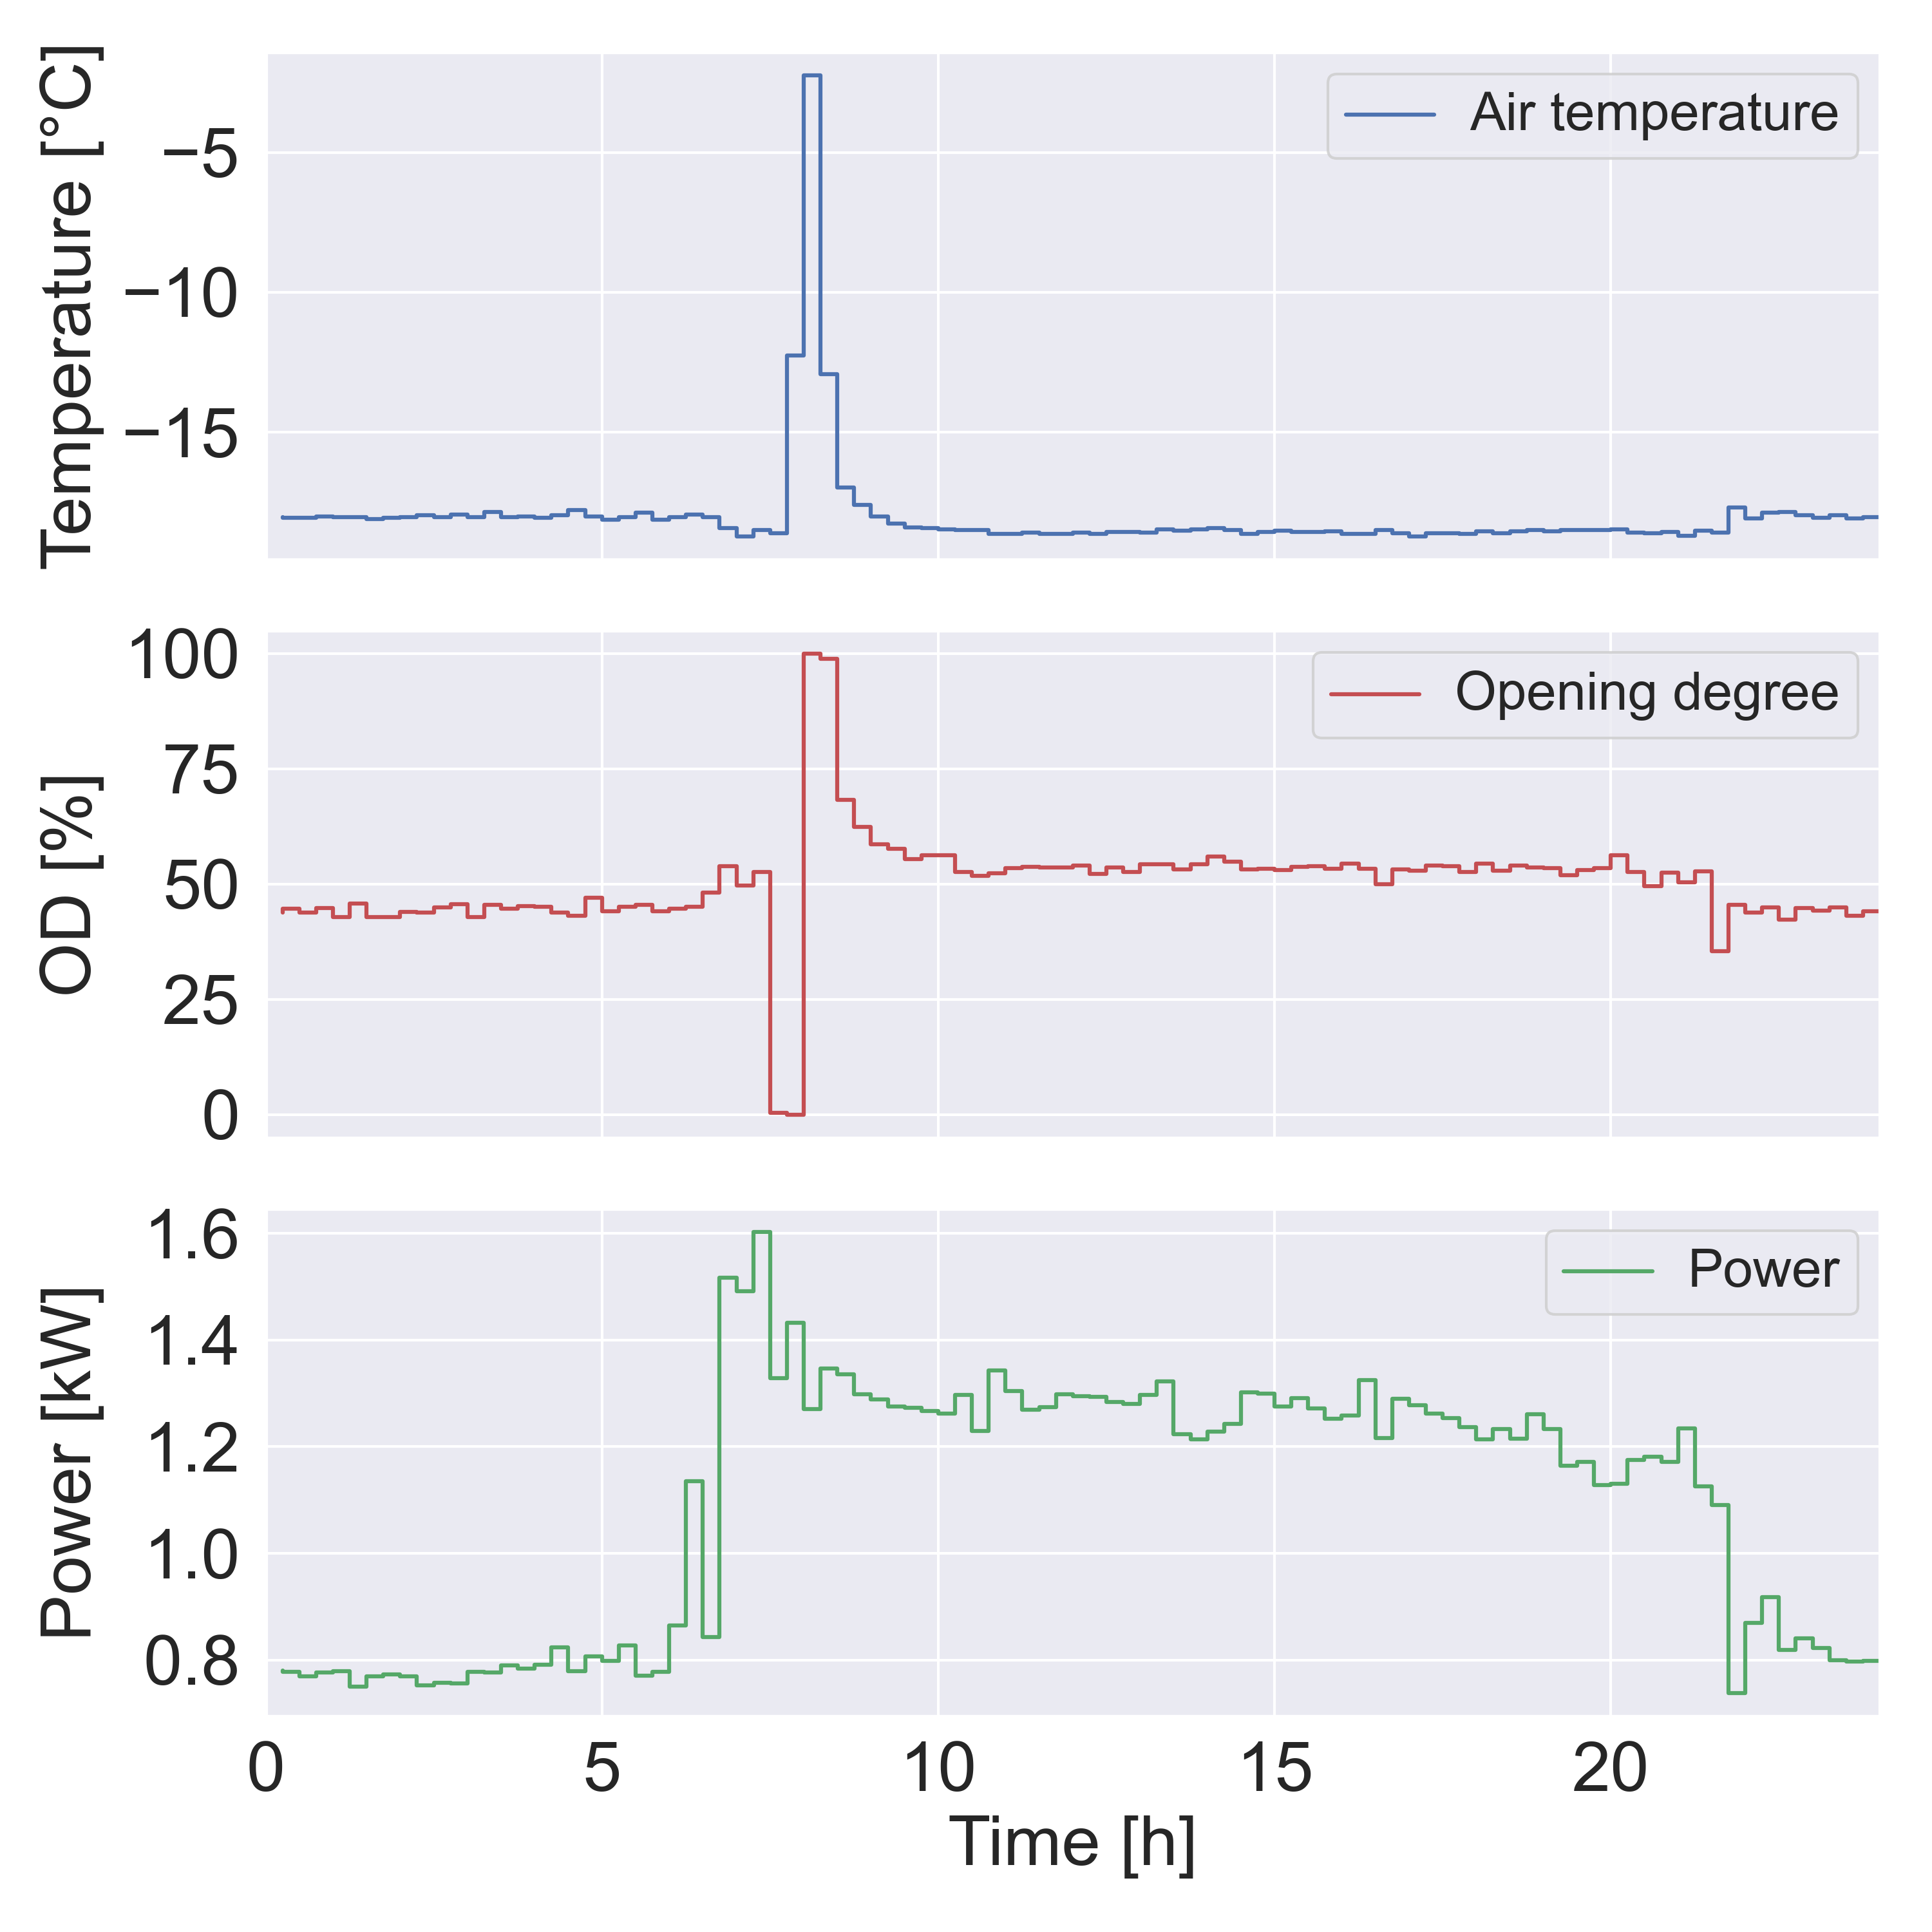
\includegraphics[width=\columnwidth]{../figures/tmp_od_Pt.png}
    \caption{\textbf{Top}: temperature of a single freezer in a supermarket. \textbf{Middle}: opening degree (OD) of the freezer expansion valve. \textbf{Bottom}: electric power of the compressor rack feeding a single freezer.}
    \label{fig:chunk}
    \vspace{-2mm}
\end{figure}

\subsubsection{Thermal modeling of freezer}

In \cite{hao2014aggregate}, it is described how a simple TCL model can be developed. We extend it to a second-order state-space model that accounts for the thermal mass of the food, which essentially provides the flexibility in freezers:
%
\begin{subequations}\label{eq:2ndFreezerStateSpace}
    \begin{align}
        T^{\rm{f}}_{t+1} & = T^{\rm{f}}_{t} + dt \cdot \frac{1}{C^{\rm{f}}}\left(\frac{1}{R^{\rm{cf}}} (T^{\rm{c}}_{t} - T^{\rm{f}}_{t}) \right)                                                                                         \\
        T^{\rm{c}}_{t+1} & = T^{\rm{c}}_t + dt \cdot \frac{1}{C^{\rm{c}}}\Bigl(\frac{1}{R^{\rm{cf}}} (T^{\rm{f}}_t - T^{\rm{c}}_t) + \frac{1}{R^{\rm{ci}}} (T^{\rm{i}}_t - T^{\rm{c}}_t)                                          \notag \\ & \mspace{50mu} - \eta \cdot OD_t P_t \Bigr) + \epsilon \mathbbm{1}^{\text{df}}_{t},
    \end{align}
\end{subequations}
%
where $T^{\rm{c}}_t$ is the measured air temperature in the freezer at time $t \in \{1 \ldots J\}$, and $T^{\rm{f}}_t$ is the food temperature which is a latent unobserved state. There is essentially a low-pass filter of the air temperature in the freezer with time constant $\tau = C^{\rm{f}} R^{\rm{cf}}$, where $C^{\rm{f}}$ and $C^{\rm{c}}$ are the thermal capacitance of the food and air in the freezer, respectively. Parameters $R^{\rm{cf}}$ and $R^{\rm{ci}}$ are the thermal resistance between food and air in the freezer, and air and indoor temperature, respectively. Furthermore, $\epsilon$ represents the temperature change when defrosting and $\mathbbm{1}^{\text{df}}_{t}$ is the indicator function for when defrosting happens. $R^{\rm{ci}}$ is either one of two values, $R^{\rm{ci}, \text{day}}$ and $R^{\rm{ci}, \text{night}}$, to capture the differences between opening hours (6am to 10pm) and closing hours (10pm to 6am). The opening degree $OD_t$, indoor air temperature $T^{\rm{i}}_t$, and power $P_t$ are exogenous inputs as the opening degree is assumed to be fixed during a demand-response event, while only $P_t$ is controllable, and the indoor air temperature is unaffected by the freezers. Parameter $\eta$ is the compressor efficiency. The model is discretized with a time step of 15 minutes, i.e., $dt = 0.25$ hours, and $J = 96$.

\subsubsection{Model validation}

Using the R library of CTSM-R \cite{juhl2016ctsmr}, all parameters in (\ref{eq:2ndFreezerStateSpace}) have been estimated as shown in Table \ref{tab:parameter_estimates}. Notice that the thermal capacitance of the air in the freezer is significantly smaller than the thermal capacitance of the food, indicating that that the food temperature changes comparatively slower. The thermal resistance between the food and air inside the freezer, $R^{\rm{cf}}$, is also significantly smaller than the thermal resistance between the air in the freezer and the indoor temperature in the supermarket, $R^{\rm{ci}}$, both during the day and night. This makes sense as the lid acts as a physical barrier insulating the freezer. Furthermore, the thermal resistance to the indoor air temperature is higher during the night, which means that less power is needed, as  observed in Fig. \ref{fig:chunk}.

% LONG FORMAT
% \begin{table}[!t]
%     \caption{Parameter Estimates of (\ref{eq:2ndFreezerStateSpace}).}
%     \label{tab:parameter_estimates}
%     \centering
%     \begin{tabular}[b]{|l|l|l|}
%         \hline
%         Parameter                   & Value & Unit            \\ \hhline{|=|=|=|}
%         $C^{\rm{f}}$                & 6.552 & kWh/$^{\circ}$C \\
%         $C^{\rm{c}}$                & 0.077 & kWh/$^{\circ}$C \\
%         $R^{\rm{cf}}$               & 5.010 & $^{\circ}$C/kW  \\
%         $R^{\rm{ci}, \text{day}}$   & 41.05 & $^{\circ}$C/kW  \\
%         $R^{\rm{ci}, \text{night}}$ & 61.25 & $^{\circ}$C/kW  \\
%         $\eta$                      & 1.561 &                 \\
%         $\epsilon$                  & 3.372 & $^{\circ}$C/h   \\ \hline
%     \end{tabular}
% \end{table}

% LONG FORMAT V2
\begin{table}[!t]
    \caption{Parameter Estimates of (\ref{eq:2ndFreezerStateSpace}).}
    \label{tab:parameter_estimates}
    \centering
    \begin{tabular}[b]{|l|l|l||l|l|l|}
        \hline
        Parameter                 & Value & Unit            & Parameter                   & Value & Unit           \\ \hhline{|=|=|=|=|=|=|}
        $C^{\rm{f}}$              & 6.552 & kWh/$^{\circ}$C & $R^{\rm{ci}, \text{night}}$ & 61.25 & $^{\circ}$C/kW \\
        $C^{\rm{c}}$              & 0.077 & kWh/$^{\circ}$C & $\eta$                      & 1.561 &                \\
        $R^{\rm{cf}}$             & 5.010 & $^{\circ}$C/kW  & $\epsilon$                  & 3.372 & $^{\circ}$C/h  \\
        $R^{\rm{ci}, \text{day}}$ & 41.05 & $^{\circ}$C/kW  &                             &       &                \\ \hline
    \end{tabular}
    \vspace{-2mm}
\end{table}

% WIDE FORMAT
% \begin{table}[!t]
%     \caption{Parameter Estimates of (\ref{eq:2ndFreezerStateSpace}).}
%     \label{tab:parameter_estimates}
%     \centering
%     \begin{tabular}[b]{|l|l|l||l|l|l||l||l|}
%         \hline
%         Parameter & $C^{\rm{f}}$ & $C^{\rm{c}}$ & $R^{\rm{cf}}$ & $R^{\rm{ci}, \text{day}}$ & $R^{\rm{ci}, \text{night}}$ & $\eta$ & $\epsilon$ \\ \hhline{|=|=|=||=|=|=|=|=|}
%         Value     & 6.552        & 0.077        & 5.010         & 41.05                     & 61.25                       & 1.561  & 3.372      \\ \hline
%     \end{tabular}
% \end{table}




The one-step residuals for the air temperature should ideally resemble white noise in order for a model to capture all dynamics seen in the data \cite{madsen2007time}. Fig. \ref{fig:2ndFreezerModelValidation} shows the auto-correlation and cumulative periodogram of the residuals. The autocorrelation shows two significant lags for lag two and seven, but looks satisfactory otherwise. Likewise,  it seems the model is able to capture most dynamics at all frequencies.
%
Since there are only 96 time steps, the defrosting period can result in relatively large residuals as it is difficult to capture such fast transient dynamics. Since up-regulation is not allowed during defrosting, the residuals are not too important during that period. To decrease their effect in the parameter estimation procedure, the term $ \epsilon \mathbbm{1}^{\text{df}}_{t}$ was added to (\ref{eq:2ndFreezerStateSpace}).

\begin{figure}[!t]
    \centering
    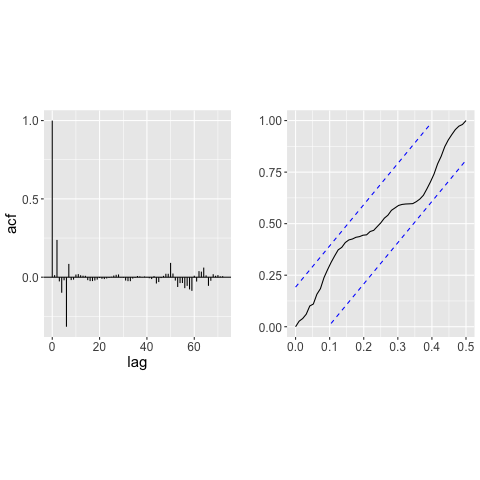
\includegraphics[width=\columnwidth]{../figures/2ndFreezerModelValidation.png}
    \caption{ Validation of the state-space model in (\ref{eq:2ndFreezerStateSpace}). \textbf{Left}: auto-correlation function (acf) of the  residuals. \textbf{Right}: cumulated periodogram of the residuals.}
    \label{fig:2ndFreezerModelValidation}
    \vspace{-1mm}
\end{figure}



Furthermore, Fig. \ref{fig:2ndFreezerModelSimulation} (left) shows a 24-hour simulation of  (\ref{eq:2ndFreezerStateSpace}). It is seen that the simulation is  reasonable and closely follows the measured air temperature, although a slight bias is seen as the simulated temperature is a bit higher. Such a visual validation is important because the model will be embedded later in an optimization model in Section \ref{sec:OptimizationModel}.

Ideally, the validation of (\ref{eq:2ndFreezerStateSpace}) would also include real measurements from the air and food temperature in a freezer during demand-response events. However, by adhering to the fundamental physics governing the temperature dynamics as shown, the model is trusted to be accurate during demand-response events too. It brings an intuitive interpretation which can be used to understand the impact on temperature during a demand-response event.
In Fig. \ref{fig:2ndFreezerModelSimulation} (right), such a simulated example of a demand-response event is shown. It can be observed how the air temperature increases when the power is turned off, and how it decreases when the power is turned back on. The food temperature is much more stable and only changes slightly, as expected. The rebound occurs until the food temperature is back to its normal value.

\begin{figure}[!t]
    \centering
    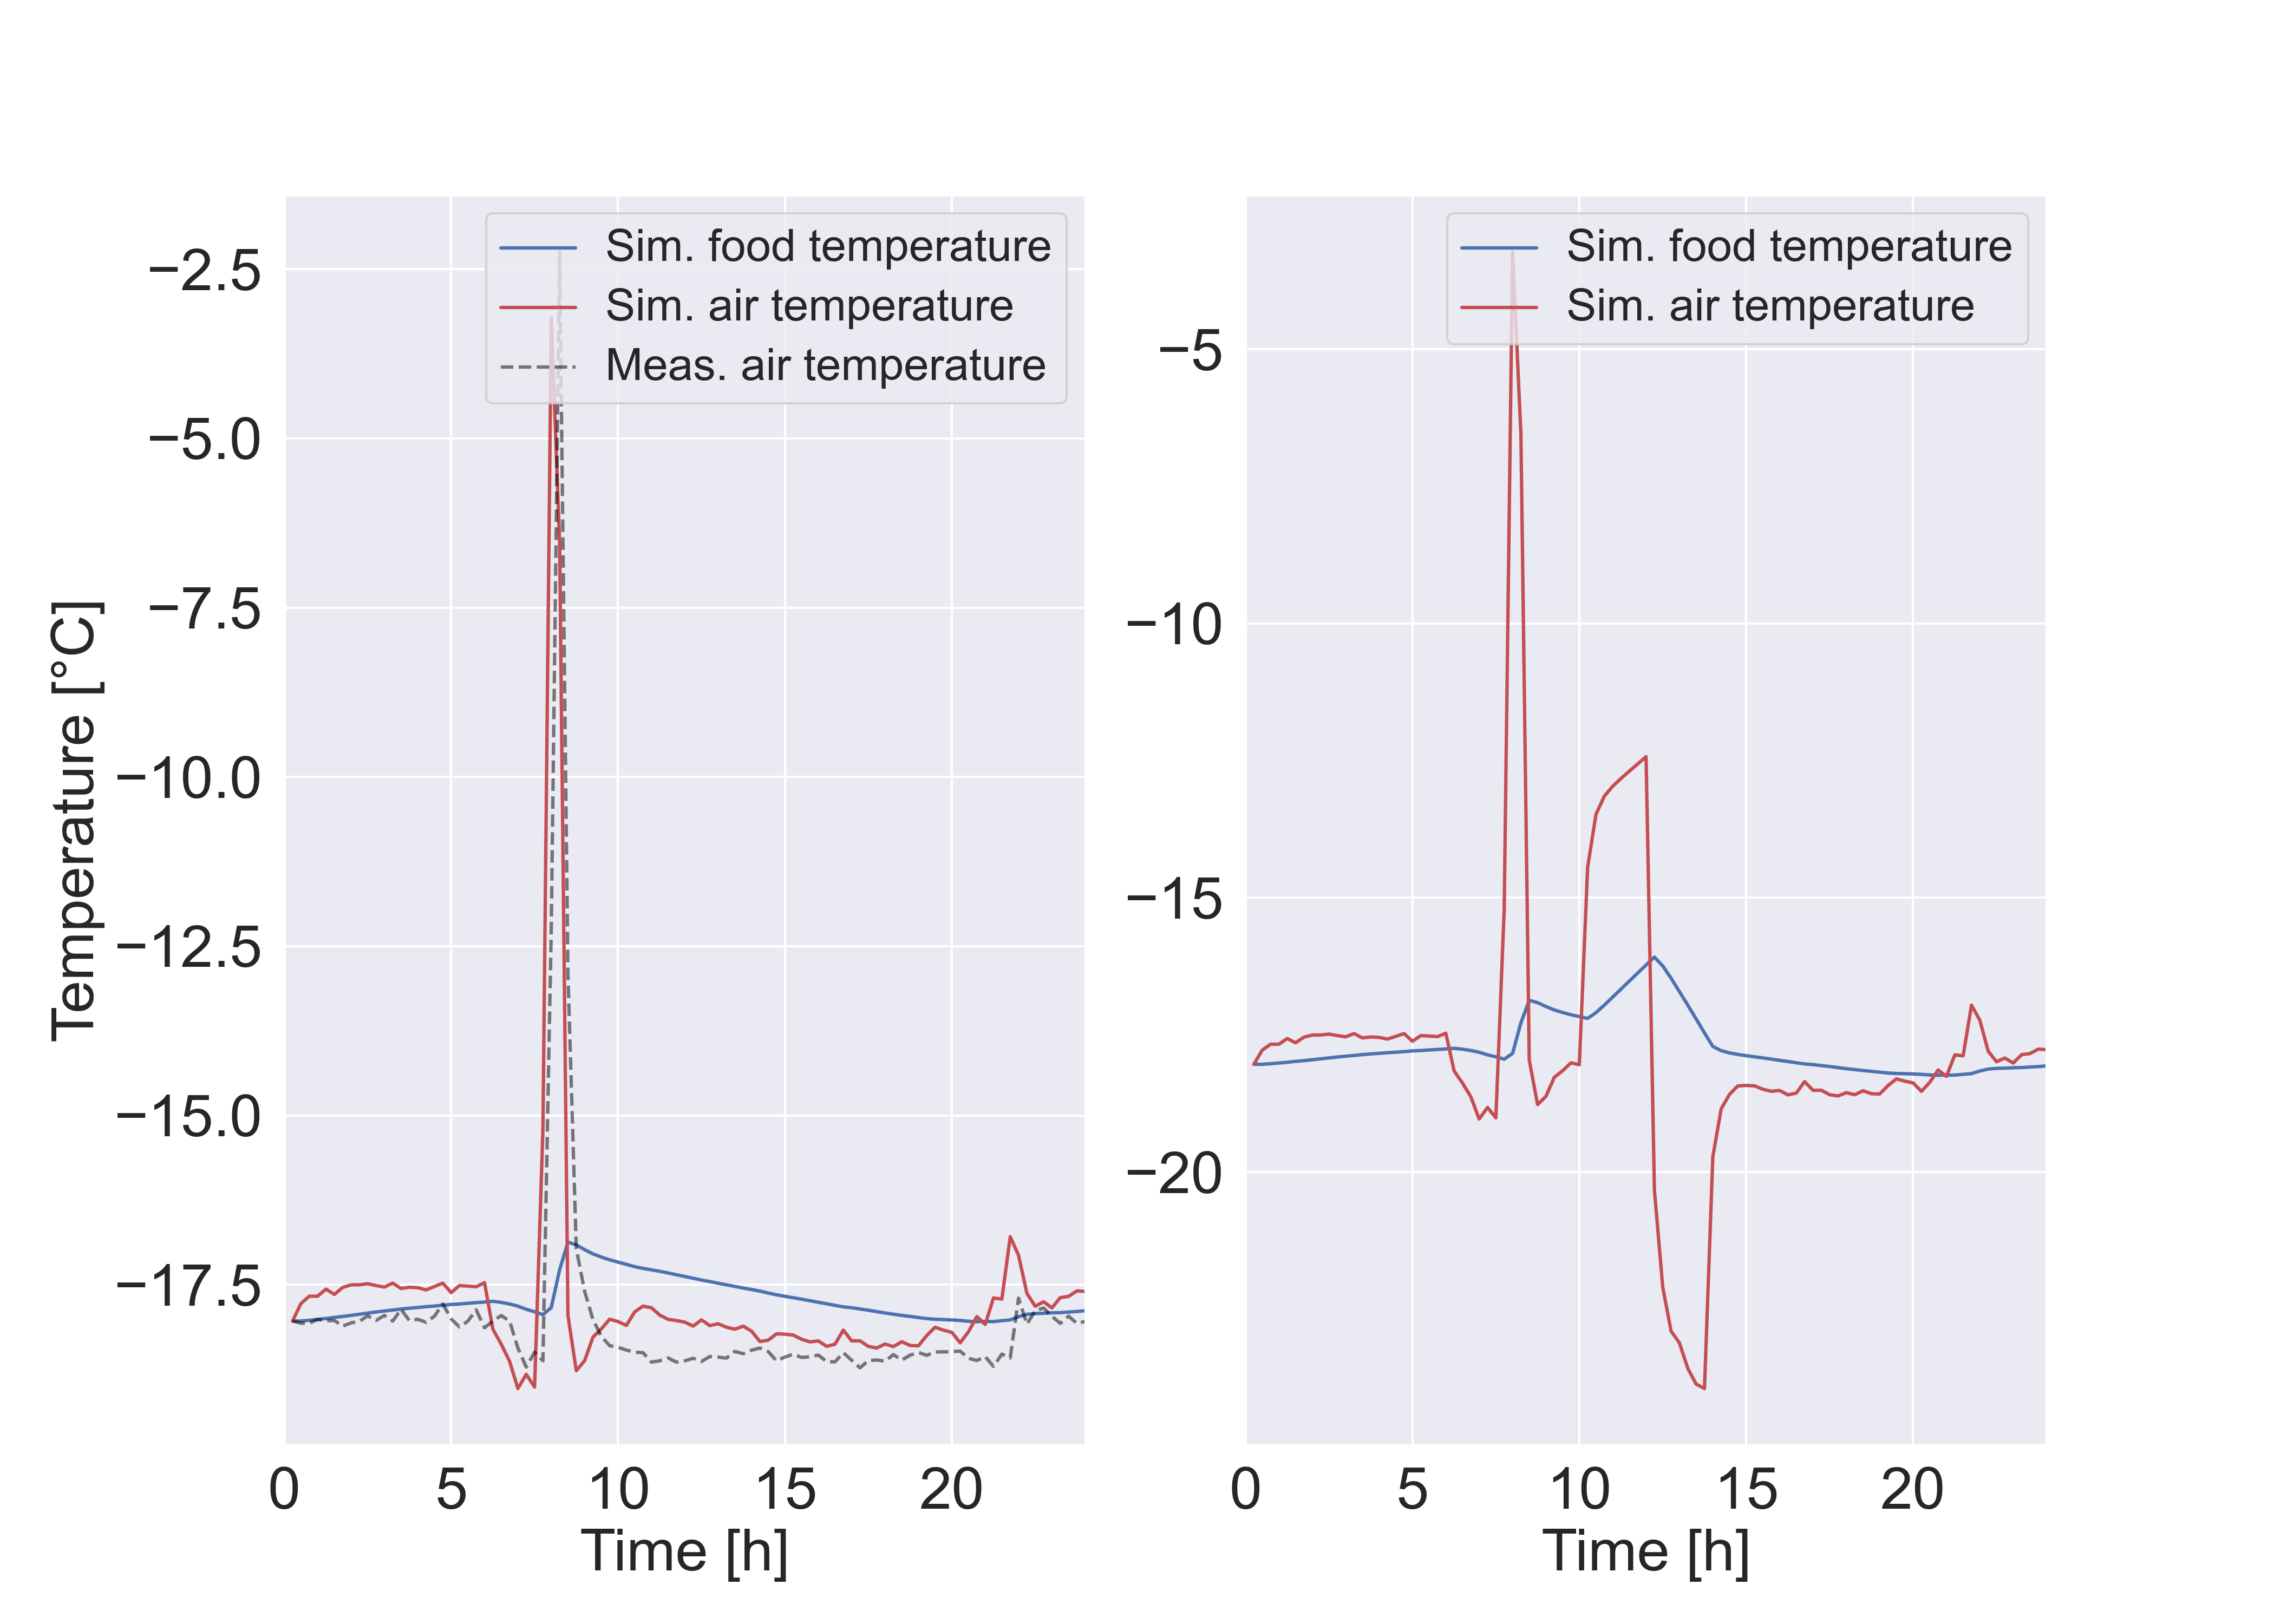
\includegraphics[width=\columnwidth]{../figures/2ndFreezerModelSimulation.png}
    \caption{ \textbf{Left}: Simulation of (\ref{eq:2ndFreezerStateSpace}) using the parameters in Table \ref{tab:parameter_estimates}. \textbf{Right}: Simulation where power is turned off for two hours with a subsequent rebound at the nominal power until the food temperature is back to its normal value.}
    \label{fig:2ndFreezerModelSimulation}
    \vspace{-2mm}
\end{figure}

\vspace{-1mm}
\subsection{mFRR}\label{sec:mFRR}
%
Fig. \ref{fig:timeline_mfrr} shows the timeline of the mFRR market in Denmark. There is a market for up-regulation only. One should note  that BRPs can choose \textit{not} to bid in the reserve market and  only bid in the real time for up- and down-regulation. We consider a case wherein the flexible demand delivers reservation through a BRP, since the payment is received for both reservation and activation. All prices considered are for the bidding zone DK2 (eastern Denmark).


\begin{figure}[!t]
    \centering
    \includestandalone[width=\columnwidth]{../figures/timeline_mfrr_tikz}
    \caption{Timeline of the Danish mFRR market. Symbols $\bm{p}$ denote power (in MW), whereas symbols  $\bm{\lambda}$ refer to price (in DKK/MW).}
    \label{fig:timeline_mfrr}
    \vspace{-3mm}
\end{figure}


The timeline for the Danish mFRR market is depicted in Fig. \ref{fig:timeline_mfrr}. At 9:30am of day $\rm{D}$-1, the BRP bids reserve capacities $p_{h}^{\rm{r},\uparrow}$ $\forall{h} \in \{1, \ldots, 24 \}$ in the mFRR market for the next day $\rm{D}$. If accepted, she is paid at the reservation price $\lambda_{h}^{\rm{r}}$. Therefore, she earns $\lambda_{h}^{\rm{r}}p_{h}^{\rm{r},\uparrow}$. This happens \textit{before} the day-ahead (spot) market clearing at noon for which the BRP buys energy for her expected demand $P_{h}^{\text{Base}}$ at the spot price $\lambda_{h}^{\rm{s}}$. After that, at 5pm, a regulating power bid, $\lambda_{h}^{\text{bid}}$, must be submitted by the BRP for each hour in $\rm{D}$, where $p_{h}^{\rm{r},\uparrow} > 0$ \cite{energinet:Systemydelser}. In hour $h$ of day $\rm{D}$, the reserves are activated if the following two conditions hold: (\textit{i}) there is a reservation accepted, i.e., $p_{h}^{\rm{r},\uparrow} > 0$, and (\textit{ii}) the balancing price $\lambda_{h}^{\rm{b}}$ is higher than both the spot price and the regulating power bid, i.e., $ \lambda_{h}^{\text{bid}} <  \lambda_{h}^{\rm{b}}$ and $ \lambda_{h}^{\rm{b}} > \lambda_{h}^{\rm{s}}$. If these conditions are met, the BRP is paid the balancing price $\lambda_{h}^{\rm{b}}$ times her actual up-regulation $p_{h}^{\rm{b},\uparrow}$. The BRP may  incur a cost due to any subsequent rebound $p_{h}^{\rm{b},\downarrow}$. Furthermore, the BRP incurs a penalty, $s_{h} = \text{max}\{0, p_{h}^{\rm{r},\uparrow} - p_{h}^{\rm{b},\uparrow}$\}, if she fails delivering her promised reserve. In reality, $p_{h}^{\rm{b},\uparrow}$ is determined by the TSO, but for simplicity, we assume a bid is always activated in its entirety.
Accordingly, the profit-maximization objective function for the BRP  for one day is
%
\begin{align}\label{eq:mFRRObjective}
    % & \underbrace{C(\text{cost})}_{\text{mFRR}} = - \underbrace{\sum_{h=1}^{24}
     & - \underbrace{\sum_{h=1}^{24} \lambda^{\rm{s}}_{h}P^{\text{Base}}_{h}}_{\textrm{Energy cost}} + \underbrace{\sum_{h=1}^{24}\lambda_{h}^{\rm{r}} p^{\rm{r}, \uparrow}_{h}}_{\textrm{Reservation payment}}  \notag \\ & \quad \quad + \underbrace{\sum_{h=1}^{24}  \lambda_{h}^{\rm{b}} p^{\rm{b},\uparrow}_{h}}_{\textrm{Activation payment}} - \underbrace{\sum_{h=1}^{24}  \lambda_{h}^{\rm{b}} p^{\rm{b},\downarrow}_{h}}_{\textrm{Rebound cost}} - \underbrace{ \sum_{h=1}^{24}  \lambda^{\rm{p}}s_{h}}_{\textrm{Penalty cost}}
\end{align}

\vspace{-2mm}
\subsection{Load shifting}
%
Another option for utilizing flexibility is to shift the load to a different time according to the spot prices which are known already 12-36 hours in advance. Then, it is simply a matter of consuming in low-price hours.
%
For a TCL, there are additional constraints to how energy can be shifted also due to the rebound. First, there can be temperature constraints which will result in less energy being shifted. Second, the rebound must happen immediately after reducing power consumption. Otherwise, the temperature deviation becomes too big for too long.
The savings from load shifting are directly proportional to the volume and price difference between the baseline load and shifted load as given by
%
\begin{equation}\label{eq:load_shifting_savings}
    \sum_{h=1}^{24} \lambda^{\rm{s}}_{h} \big(p^{\text{Base}}_{h} -  p_{h}\big),
\end{equation}
%
where $p_{h}$ is the power profile during load shifting, whereas $p^{\text{Base}}_{h}$ is the baseline.

Since the load shifting action only occurs \textit{after} the day-ahead market clearing (cf. Fig. \ref{fig:timeline_mfrr}), the BRP has already bought $\lambda^{\rm{s}}_{h} p^{\text{Base}}_{h}$ and any deviation results in an imbalance for the BRP. In this work, we look at the case where the flexible demand acts selfishly and excludes the BRP from her load shifting action. Therefore, the objective function for the flexible demand is simply $\sum_{h=1}^{24} \lambda_{h}^{\rm{s}} p_{h}$.

%\begin{equation}\label{eq:LoadShiftingObjective}
% \underbrace{C(\text{cost})}_{\text{load shifting}} = \sum_{h=1}^{24} \lambda_{h}^{\rm{s}} p_{h}
%    \sum_{h=1}^{24} \lambda_{h}^{\rm{s}} p_{h}
%\end{equation}


\section{Optimization model and solution strategy}\label{sec:OptimizationModel}
%
This section presents the optimization problem. The rest of this section is organized as follows. First, the time sequence of decisions for participation in the mFRR market is presented. Second, we explain how scenarios for price data are generated. Third, we present the model formulation. Fourth, we discuss how the bidding policy is implemented. Lastly, we show how a scenario decomposition method with an ADMM strategy is used to solve the optimization model.

\vspace{-1mm}
\subsection{Time sequence for decision making}
Fig. \ref{fig:timeline_mfrr_variables} shows the stages for making decisions in the mFRR market. In the first stage in day $\rm{D}$-1, the BRP makes a reservation bid decision $p_{h}^{\rm{r},\uparrow}$ for every hour $h$ of day $\rm{D}$,  while being uncertain about input parameters in the next stages, including day-ahead market prices $ \lambda_{h}^{\rm{s}}$  and balancing market prices $ \lambda_{h}^{\rm{b}}$. We assume the BRP is not uncertain about mFRR market prices $ \lambda_{h}^{\rm{r}}$. 

For simplicity and avoid the need for developing a multi-stage stochastic program, we merge the second, third, and fourth stages in Fig. \ref{fig:timeline_mfrr_variables} as one, and call it the second stage. By this, $p_{h}^{\rm{r},\uparrow}$ is the first-stage variable, whereas the second stage variables, indexed by scenario $\omega$, include
the regulating power bid $\lambda_{h,\omega}^{\rm{bid}}$ and the set of real-time variables $\Gamma_{h,\omega} = \{ p_{h,\omega}, p_{h,\omega}^{\rm{b},\uparrow}$, $p_{h,\omega}^{\rm{b},\downarrow}$, $s_{h,\omega}$, $T_{h,\omega}^{\rm{c}}$, $T_{h,\omega}^{\rm{f}}$, $T_{h,\omega}^{\rm{c,\text{Base}}}$, $T_{h,\omega}^{\rm{f,\text{Base}}}$, $\phi_{h,\omega}$, $g_{h,\omega}, u^{\uparrow}_{h,\omega}, u^{\downarrow}_{h,\omega}, y^{\uparrow}_{h,\omega}, y^{\downarrow}_{h,\omega}, z^{\uparrow}_{h,\omega}, z^{\downarrow}_{h,\omega} \}$. This set contains the real-time power activated, as well as auxiliary variables for identifying up- and down-regulation,  temperature dynamics, and when to deliver up-regulation according to the bid and prices. See the Appendix for a detailed description. Note that down-regulation refers to the rebound effect of the freezer.
% \begin{figure}[!t]\label{fig:timeline_mfrr_variables}
%     \centering
%     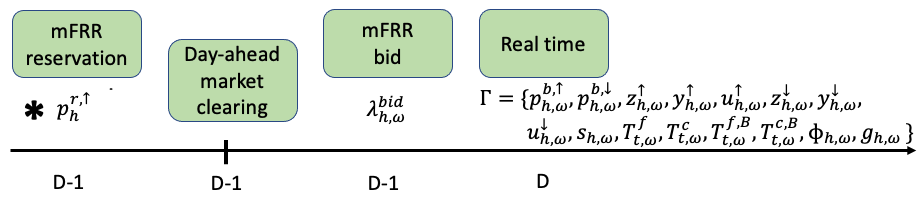
\includegraphics[width=\columnwidth]{../figures/timeline_mfrr_variables.png}
%     \caption{Variables related to mFRR up-regulation decisions. The asterisk indicates the first-stage decision.}
% \end{figure}

\begin{figure}[b]
    \centering
    \includestandalone[width=\columnwidth]{../figures/timeline_mfrr_variables_tikz}
    \caption{Variables related to the mFRR  bidding decisions.}
    \label{fig:timeline_mfrr_variables}
\end{figure}

\vspace{-1mm}
\subsection{Scenario generation}\label{sec:scenario_generation}
To make decisions on reservation capacity $p_{h}^{\rm{r},\uparrow}$ and regulating power bid $\lambda_{h,\omega}^{\rm{bid}}$, we generate a set of scenarios $\omega \in \Omega$ for spot and balancing price data., i.e., $ \lambda_{h,\omega}^{\rm{s}}$ and $ \lambda_{h,\omega}^{\rm{b}}$. Each scenario contains spot and balancing price data for the entire day in question. The number of scenarios is $|\Omega|$, and we assume all scenarios are equiprobable. We refer to them as \textit{in-sample} scenarios. We use two different strategies for in-sample scenario generation: (\textit{i}) considering historical spot and balancing prices in DK2 in 2021.
%, with different cases where the number of scenarios $|\Omega|$ is 1, 5, 10, 20, 30, 40, 50, 100, and 250. 
(\textit{ii}) considering prices of the most recent five days (lookback strategy). In both scenario generation strategies, balancing prices $\lambda_{h,\omega}^{\rm{b}}$ are sampled in the following way: First, an integer $v$ is sampled uniformly from $\{0, \ldots, 24\}$ which represents the total number of up-regulation hours in a day. We then sample spot and balancing price differentials from a single day within the set of all days where up-regulation happened $v$ times. This constitutes one scenario and is repeated $|\Omega|$ times. In this way, days where up-regulation happened are essentially up-sampled, and the model learns more when up-regulation happens than otherwise. The in-sample results are systematically compared against the same set of unseen \textit{Out-of-Sample} (OOS) scenarios, which are DK2 prices for 2022.

For load shifting, the solution approach is simply to solve a deterministic optimization problem for the next day, since the day-ahead (spot) market clearing happens in advance, and thereby the spot market prices are known.

\vspace{-1mm}
\subsection{Model formulation}
Recall that \eqref{eq:mFRRObjective} gives the objective function of a BRP participating in the mFRR market, but in a deterministic setup.  The optimization problem of such a BRP in a two-stage stochastic programming format is
%
\begin{subequations}\label{P1:compact_model}
    \begin{align}
        \underset{\bm{p}^{\rm{r},\uparrow}, \bm{\lambda}_{\omega}^{\rm{bid}}, \bm{\Gamma}_{\omega}}{\text{Maximize}} \ & f(\bm{p}^{\rm{r},\uparrow}) + \sum_{\omega \in \Omega} \pi_{\omega} \ g(\bm{\Gamma}_{\omega}) \label{P1:eq1}
        \\
        \text{s.t.} \                                                                                            & h(\bm{p}^{\rm{r},\uparrow}, \bm{\lambda}_{\omega}^{\rm{bid}}, \bm{\Gamma}_{\omega}) \leq 0, \ \forall{\omega}\label{P1:eq2}                                                                                             \\
        \                                                                                                        & \text{State-space model } (\ref{eq:2ndFreezerStateSpace}), \ \forall{\omega} \label{P1:eq3}
        \\
        \                                                                                                        & \bm{T}_{\omega}^{\rm{c}}, \bm{T}_{\omega}^{\rm{f}},  \bm{T}_{\omega}^{\rm{c,\text{Base}}}, \bm{T}_{\omega}^{\rm{f,\text{Base}}}\in \mathbb{R}  \label{P1:eq4}
        \\
                \                                                                                                        & \bm{p}_{\omega}, \bm{p}^{\rm{r},\uparrow}, \bm{\lambda}_{\omega}^{\rm{bid}}, \bm{p}_{\omega}^{\rm{b},\uparrow}, \bm{p}_{\omega}^{\rm{b},\downarrow}, \bm{s}_{\omega},  \bm{\phi}_{\omega}\in \mathbb{R}^{+}  \label{P1:eq5}
        \\
        \                                                                                                        & \bm{g}_{\omega}, \bm{u}^{\uparrow}_{\omega}, \bm{z}^{\uparrow}_{\omega}, \bm{y}^{\uparrow}_{\omega}, \bm{u}^{\downarrow}_{\omega}, \bm{z}^{\downarrow}_{\omega}, \bm{y}^{\downarrow}_{\omega} \in \{0,1\},  \label{P1:eq6}
    \end{align}
\end{subequations}
%
where bold symbols represent vectors. For example, the vector $\bm{p}^{\rm{r},\uparrow}$ includes $p_{h}^{\rm{r},\uparrow} \ \forall{h}$. Parameter $\pi_{\omega}$ is the probability assigned to in-sample scenario $\omega$. Here, we present optimization \eqref{P1:compact_model} in a compact form using functions $f(.)$, $g(.)$, and $h(.)$. The detailed formulation is given in the Appendix. Constraint (\ref{P1:eq2}) includes all power and activation related limits, whereas (\ref{P1:eq3}) models temperature dynamics in the freezer. Constraints (\ref{P1:eq4})-(\ref{P1:eq5}) declare continuous and binary variables. Note that $\mathbb{R}$ and $\mathbb{R}^{+}$ denote free and non-negative real numbers, respectively. The optimization model \eqref{P1:compact_model} is a MILP problem.


For optimal decision making for load shifting, \eqref{P1:compact_model} is simplified by removing scenarios as well as reservation and bid constraints, and replacing the objective function (\ref{P1:eq1}) by minimizing the total power purchase cost $\bm{\lambda}^{\rm{s}} \bm{p}$.

\vspace{-1mm}
\subsection{Regulating power bidding implementation}\label{sec:mFRR_bidding_implementation}
Recall from  Fig. \ref{fig:timeline_mfrr_variables} that we have merged three stages, by which the regulating power bidding decisions $\lambda_{h,\omega}^{\rm{bid}}$ and real-time operational decisions $\Gamma_{h,\omega}$ become second-stage variables. This is the reason both set of variables $\lambda_{h,\omega}^{\rm{bid}}$ and $\Gamma_{h,\omega}$ are similarly indexed by $\omega$, while in reality, the decision $\lambda_{h,\omega}^{\rm{bid}}$ should be made before $\Gamma_{h,\omega}$. This also challenges the ex-post OOS simulation. To resolve it, we use a learning policy, such that we replace the scenario-indexed variable $\lambda_{h,\omega}^{\rm{bid}}$ in \eqref{P1:compact_model} by $\alpha q(\lambda_{h,\omega}^{\rm{s}}) + \beta$, where $q(.)$ is an arbitrarily selected function. In addition, $\alpha$ and $\beta$ are non-negative first-stage  variables (they are not indexed by $\omega$). This replacement shrinks the degree of freedom for the BRP compared to \eqref{P1:compact_model}, but makes it more practical to be used. The reason is that, by this trick, the regulating power bidding decision to be made at 5pm of day $\rm{D}$-1 becomes a first-stage decision, dependent not only on policies $\alpha$ and $\beta$, but also on uncertain spot prices $\lambda_{h,\omega}^{\rm{s}}$. In other words, by using the in-sample scenarios $\omega$, the BRP obtains optimal values for $\alpha$ and $\beta$ at 9:30am of day $\rm{D}$-1. Then, she waits to see the spot prices at noon of day $\rm{D}$-1, and  submits her regulating power bids at 5pm of day $\rm{D}$-1. In our simulations, we found out that the selection of $q(\lambda_{h,\omega}^{\rm{s}})$ as the difference of spot prices in subsequent hours works comparatively more satisfactory ex-post, as it suits better to accommodate the rebound effect. By this, the BRP prefers to be activated when the spot price during rebound (down-regulation) is comparatively lower. Therefore, we replace $\lambda_{h,\omega}^{\rm{bid}}$ in \eqref{P1:compact_model} by
%
\begin{align}\label{eq:affine_policy}
     & \alpha ( \lambda_{h+1,\omega}^{\rm{s}} - \lambda_{h,\omega}^{\rm{s}}) + \lambda_{h,\omega}^{\rm{s}} + \beta, \ \forall{\omega}, \forall{h} \in \{1, \ldots, 23\}.
\end{align}



%To solve Problem (\ref{P1:compact_model}), we first need to specify a bidding policy that can readily be used OOS. We do so by choosing an affine bidding policy. Afterwards, it is shown how the bidding policy is implemented using McCormick relaxation.

%\subsubsection{Affine bidding policy}

%A bidding policy needs to be easy to follow OOS for the trader. We choose an affine bidding policy, i.e., a linear function of the spot price. The bidding policy is given by:





%Variables $\alpha$ and $\beta$ are then learned IS and fixed for OOS evaluation. After the day-ahead market clearing, (\ref{eq:affine_policy}) can easily be used to specify bids for the next day.

Another implementation challenge is to enforce price conditions under which the mFRR reservation is activated.
Recall from Section \ref{sec:mFRR}, for the activation at hour $h$ under scenario $\omega$, it is necessary to hold $\lambda_{h,\omega}^{\rm{bid}} \leq  \lambda_{h,\omega}^{\rm{b}} - \lambda_{h,\omega}^{\rm{s}}$ and $ \lambda_{h,\omega}^{\rm{b}} > \lambda_{h,\omega}^{\rm{s}}$. These conditions can be equivalently enforced as
%
%activation of mFRR reservation only happens when certain price conditions are met. This is formalized in the following constraint:
%
\begin{equation}\label{eq:bid_constraint}
    p^{\rm{b}, \uparrow}_{h,\omega} + s_{h,\omega} \geq p^{\rm{r},\uparrow}_{h}  \mathbbm{1}^{\big(\lambda_{h,\omega}^{\rm{bid}} \leq  \lambda_{h,\omega}^{\rm{b}} - \lambda_{h,\omega}^{\rm{s}} \ \text{and} \ \lambda^{\rm{b}}_{h,\omega} > \lambda^{\rm{s}}_{h,\omega}\big)},
\end{equation}
where $\mathbbm{1}^{(.)}$ is 1 if conditions (.) are met, otherwise it is zero. If the non-negative slack variable $s_{h,\omega}$ takes a non-zero value, it shows that the BRP fails in the activation stage, and therefore will be penalized. The challenge is that \eqref{eq:bid_constraint} makes a condition on variable $\lambda_{h,\omega}^{\rm{bid}}$, or equivalently on $\alpha$ and $\beta$ as defined in \eqref{eq:affine_policy}. This makes \eqref{eq:bid_constraint} non-linear. To linearize it, we use the McCormick relaxation technique \cite{mccormick1976computability} and define auxiliary  variables $\phi_{h,\omega} \in \mathbb{R}^{+}$ and $g_{h,\omega} \in \{0, 1\}$. By this, we replace \eqref{eq:bid_constraint} for every hour $h$ and scenario $\omega$ by a set of mixed-integer linear constraints as
%
%Eq. (\ref{eq:bid_constraint}) shows how real-time up-regulation plus a slack variable must be greater than or equal to the reservation if the bid is lower than the balancing price and if up-regulation is needed in hour $h$. It is a bi-linear constraint so McCormick relaxation \cite{mccormick1976computability} is used to convert (\ref{eq:bid_constraint}) to a linear constraint by introducing auxiliary variables, $\phi_{h,\omega}$ and $g_{h,\omega}$:
%
\begin{subequations}\label{eq:bid_constraint_relaxed}
    \begin{align}
       & \lambda_{h,\omega}^{\rm{bid}} - M  (1 - g_{h,\omega}) \leq \lambda_{h,\omega}^{\rm{b}} - \lambda_{h,\omega}^{\rm{s}} \leq \lambda_{h,\omega}^{\rm{bid}} + M  g_{h,\omega},                               \label{con_bid:subeq1}\\
        & p^{\rm{b}, \uparrow}_{h,\omega} \leq \phi_{h,\omega}  \mathbbm{1}^{\lambda^{\rm{b}}_{h,\omega} > \lambda^{\rm{s}}_{h,\omega}}, \                          \label{con_bid:subeq3}  \\
        &p^{\rm{b}, \uparrow}_{h,\omega} + s_{h,\omega} \geq \phi_{h,\omega}  \mathbbm{1}^{\lambda^{\rm{b}}_{h,\omega} > \lambda^{\rm{s}}_{h,\omega}}, \            \label{con_bid:subeq4}  \\
        &-g_{h,\omega}  M \leq \phi_{h,\omega} \leq g_{h,\omega}  M,                                   \label{con_bid:subeq5}  \\
        &-(1 - g_{h,\omega})  M \leq \phi_{h,\omega} - p^{\rm{r},\uparrow}_{h} \leq (1 - g_{h,\omega}) M, \                                                                                    \label{con_bid:subeq7}  \
        % \lambda_{h,\omega}^{\rm{bid}} \leq \lambda^{Max} \label{con_bid:subeq9}
    \end{align}
\end{subequations}
where $M$ is a large enough positive constant.
Constraint \eqref{con_bid:subeq1} ensures that $g_{h,\omega} = 1$ when $\lambda_{h,\omega}^{\rm{b}} - \lambda_{h,\omega}^{\rm{s}} \geq \lambda^{\rm{bid}}_{h, \omega}$. Otherwise, it sets $g_{h,\omega} = 0$. Constraints \eqref{con_bid:subeq3}-\eqref{con_bid:subeq4} set the up-regulation equal to $\phi_{h,\omega}$ (or incurs a penalty through $s_{h,\omega}$) if there is an up-regulation event in the system, i.e., if $\mathbbm{1}^{\lambda^{\rm{b}}_{h,\omega} > \lambda^{\rm{s}}_{h,\omega}} = 1$. Constraint \eqref{con_bid:subeq5} enforces  $\phi_{h,\omega} = 0$ when $g_{h,\omega} = 0$, implying the balancing price minus the spot price is smaller than the power regulating bid. Constraint \eqref{con_bid:subeq7} ensures that $\phi_{h,\omega}$ is equal to the reservation capacity $p^{\rm{r},\uparrow}_{h}$ whenever $g_{h,\omega} = 1$, i.e., if $\lambda_{h,\omega}^{\rm{b}} - \lambda_{h,\omega}^{\rm{s}} \geq \lambda^{\rm{bid}}_{h, \omega}$. Note that in the final model,  $\lambda^{\rm{bid}}_{h, \omega}$ in \eqref{eq:bid_constraint_relaxed} should be replaced as defined in \eqref{eq:affine_policy}. The resulting model formulation, which is a MILP, is given in the Appendix.

\vspace{-1mm}
\subsection{Scenario decomposition with ADMM}
By increasing the number of scenarios,  the proposed stochastic program  quickly becomes computationally intractable due to the number of binary variables and intertemporal constraints. To resolve it, we apply a scenario decomposition approach built upon the ADMM algorithm \cite{boyd2011distributed}. To do so, we relax non-anticipativity constraints by adding a scenario index to the first-stage variables, i.e.,
%
\begin{equation}\label{eq:non_anticipativity}
    p_{h}^{\rm{r},\uparrow} \rightarrow p^{\rm{r},\uparrow}_{h,\omega}, \ \alpha \rightarrow \alpha_{\omega}, \ \beta \rightarrow \beta_{\omega}.
\end{equation}

This decomposes the original problem to a set of deterministic sub-problems, one per scenario, to be solved in parallel. A quadratic regularizer is added to the objective function of every subproblem, making it a mixed-integer quadratic program.  
The ADMM algorithm is iterative. The convergence happens when we achieve a consensus over sub-problems on first-stage  variables. Due to having binary variables in the original problem, this ADMM algorithm is eventually a heuristic \cite{hong2016convergence}, i.e., it may not converge to optimality. However, we have observed in a case with a limited number of scenarios for which we can also solve the original MILP problem directly, the proposed ADMM exhibits a satisfactory performance.



\section{Numerical Results and Discussion}\label{sec:results}
In this section, we present and discuss the results related to providing mFRR versus load shifting for a single supermarket freezer using the optimization model in (\ref{P1:compact_model}), and the scenarios and solution strategies described in Sections \ref{sec:scenario_generation} and \ref{sec:mFRR_bidding_implementation}. First, we discuss the main result: mFRR versus load shifting. Second, we discuss the effectiveness of the ADMM solution strategy using 2021 price data.

\subsection{Load shifting vs mFRR}
Figure \ref{fig:cumulative_cost_comparison} shows the cumulative cost of operation for mFRR versus load shifting compared to the baseline cost. For mFRR, the lookback strategy is similar to ADMM strategy using 2021 scenarios. But both of them have a higher cost than load shifting for most of the year. Interestingly, mFRR was very profitable in June (reservation prices increased significantly due to an outage of a reserve power plant).

\begin{figure}[!t]
    \centering
    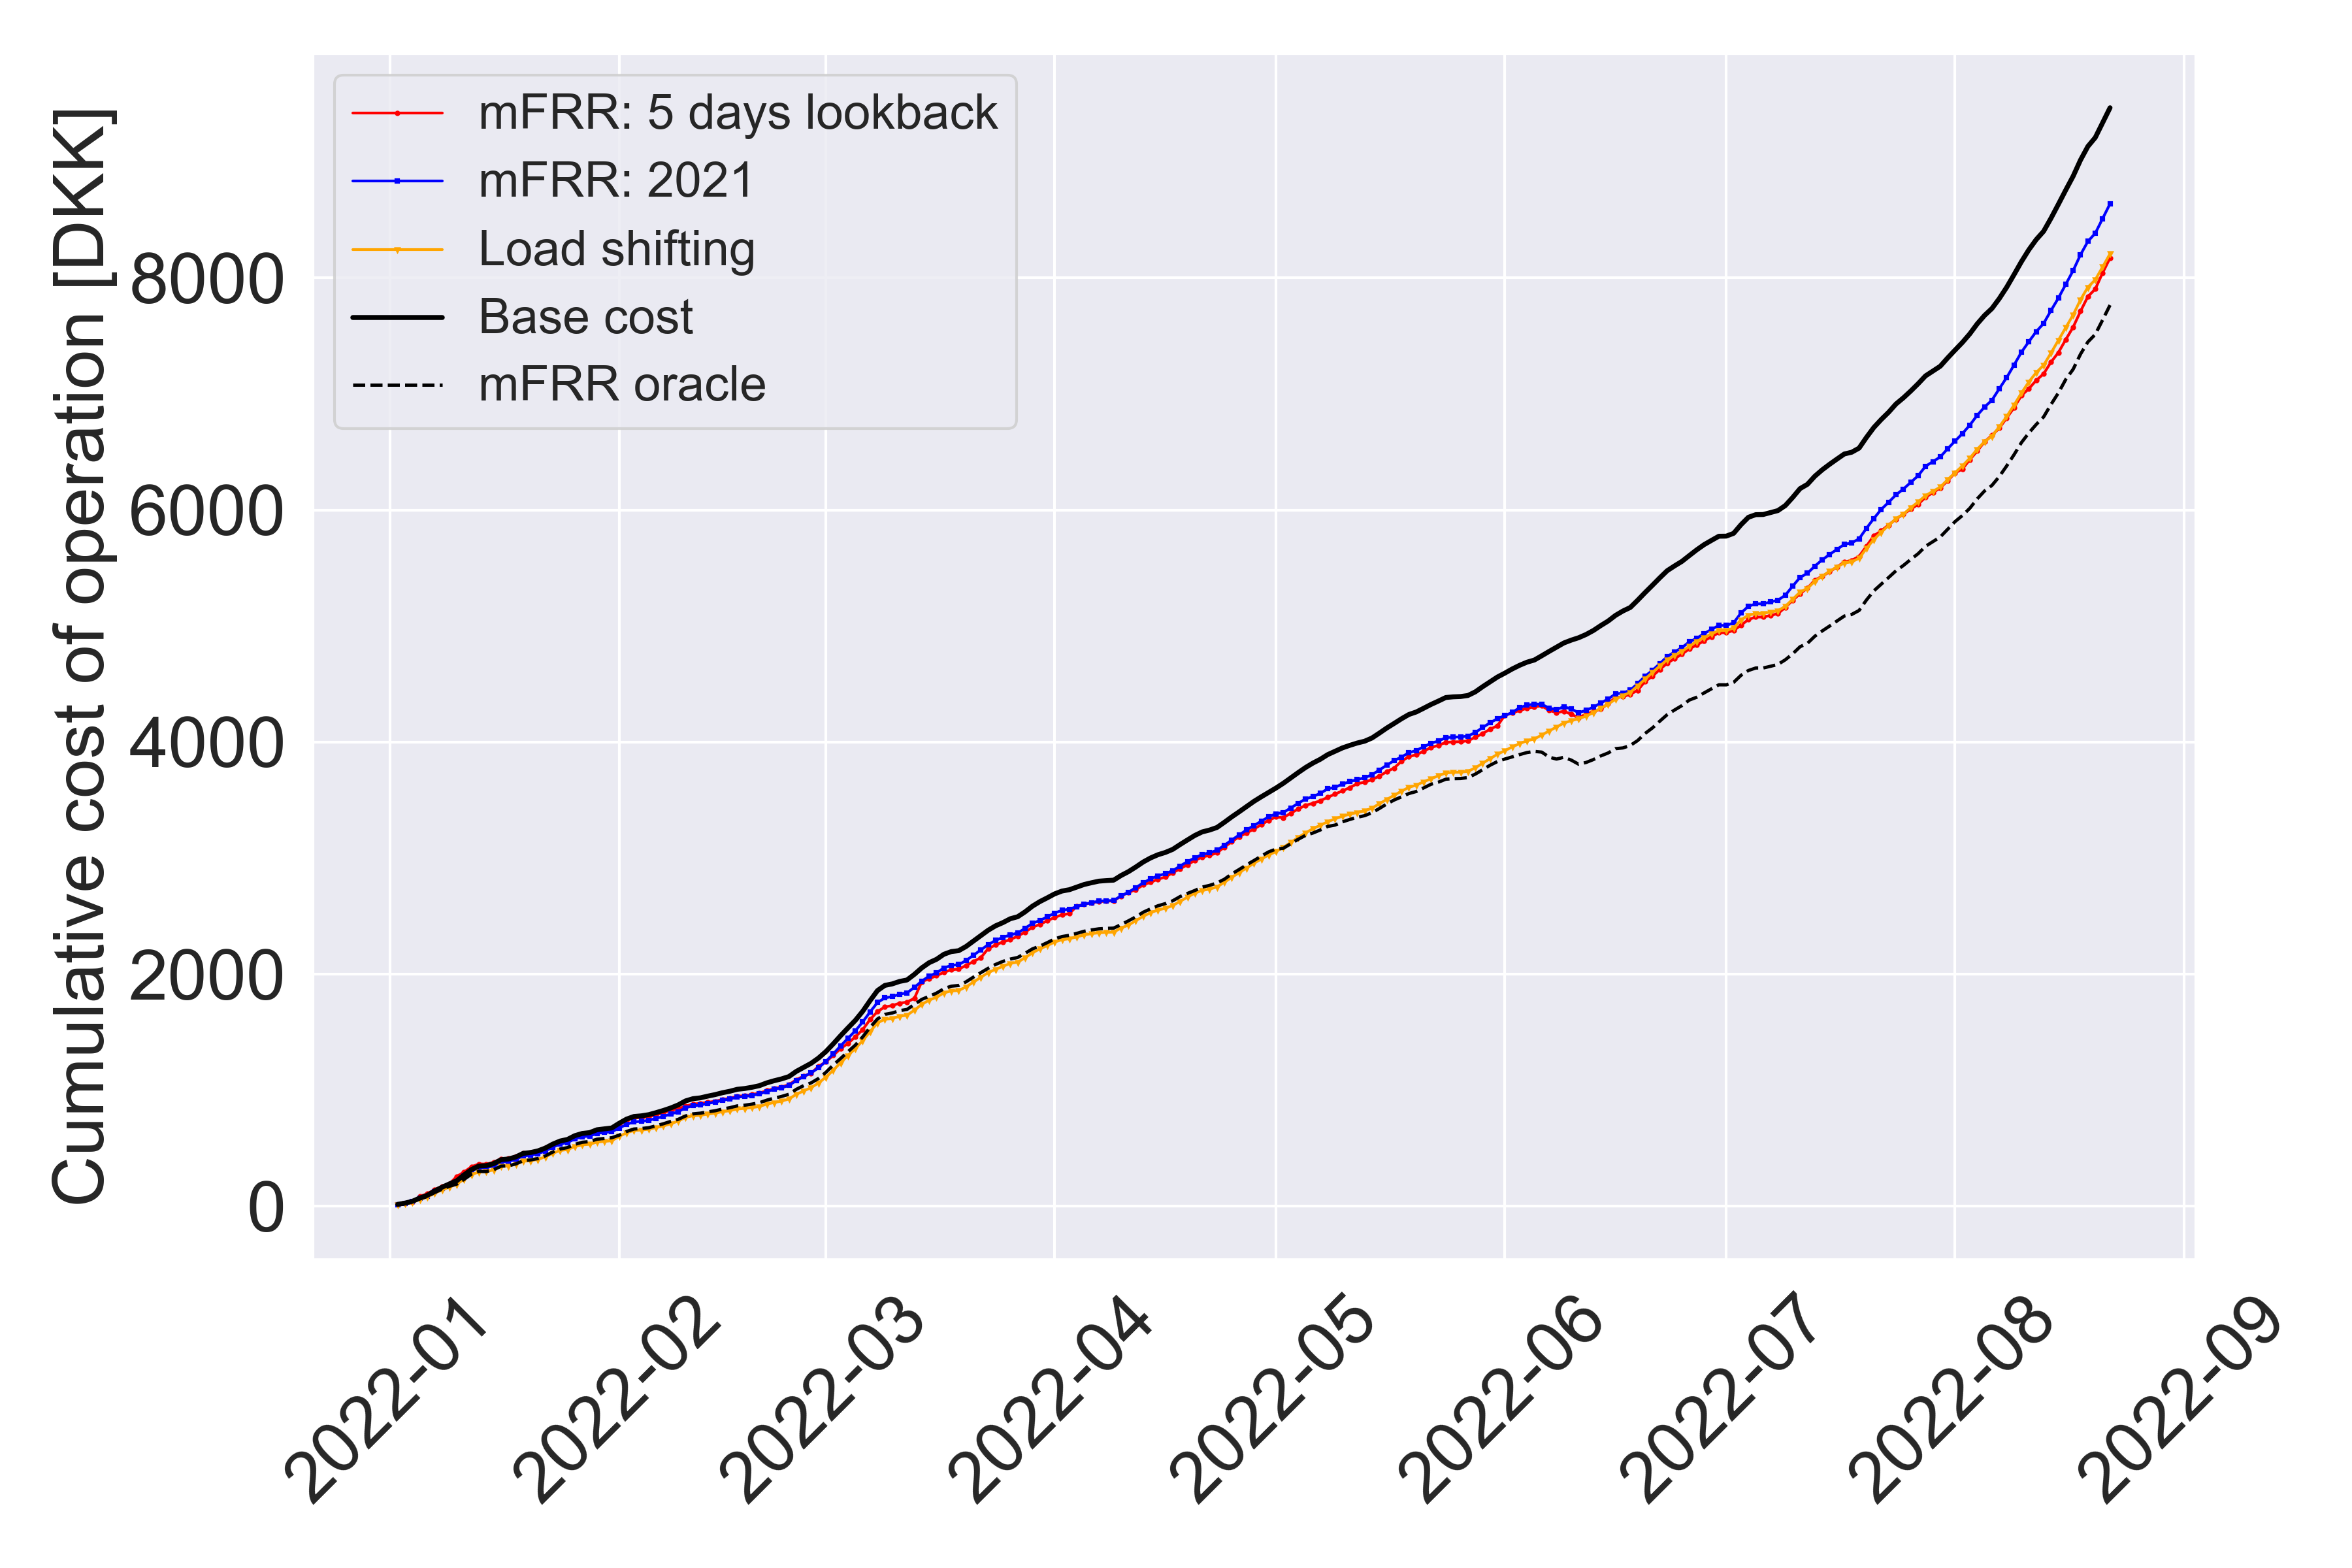
\includegraphics[width=\columnwidth]{../figures/cumulative_cost_comparison.png}
    \caption{OOS cumulative cost of operation for load shifting and mFRR using ADMM with 50 scenarios trained on 2021 data (blue), and a lookback of five days (red). Base costs are also shown together with an oracle that has full hindsight on prices.}
    \label{fig:cumulative_cost_comparison}
\end{figure}

Table \ref{tab:cases_compared} breaks down the cost components. For mFRR, there is big difference between the lookback strategy and the ADMM strategy with 2021 prices. The lookback strategy earns much more from activation payments, but is also penalized more as it is not able to deliver its reservation capacity in some days. The other mFRR strategy bids more conservatively and is only rarely activated. The market rules prescribe that the full bid should be delivered, hence the lookback strategy might be too risky. On the other hand, it was assumed that the activation power should be equal to the reserved power, but the TSO determines the activation power, hence the activation power might be lower in reality which would both decrease the penalty cost and the activation revenue.

All strategies are better than the baseline costs, i.e., not utilizing flexibility, with savings of 10-14\%. Furthermore, the mFRR strategies are not far off the theoretically best mFRR strategy as indicated by the oracle in Figure \ref{fig:cumulative_cost_comparison}.

\begin{flushleft}
    \begin{table}[!t]
        \caption{Average Daily OOS Costs.}
        \label{tab:cases_compared}
        \centering
        \begin{tabular}{lccc}
            \toprule
            Name                 & \thead{mFRR w.                   \\lookback} & Load shifting & \thead{mFRR \\w. 2021} \\
            \midrule
            Base cost today      & 40.628         & 40.628 & 40.628 \\
            Total cost           & 35.918         & 34.994 & 36.514 \\
            Expected energy cost & 40.628         & 34.994 & 40.628 \\
            Rebound cost         & 0.858          & N/A    & 0.911  \\
            Reserve payment      & 3.216          & 0.0    & 3.381  \\
            Act payment          & 8.092          & 0.0    & 2.161  \\
            Penalty cost         & 5.741          & 0.0    & 0.516  \\
            Scenarios            & -5             & 1      & 50     \\
            ADMM                 & False          & False  & True   \\
            \% savings           & 11.6           & 13.9   & 10.1   \\
            \bottomrule
        \end{tabular}
    \end{table}
\end{flushleft}

In Figure \ref{fig:fig_sim}, load shifting and mFRR are compared for the same day. For load shifting, it can clearly be seen how load is shifted to low-price hours, especially at the end of the day. But it also has a very significant effect on the temperature with large deviations from its normal setpoint. For mFRR, the reservation is almost full for all hours during the day. The activation of reservation occurs when the bid price is lower than the balancing price which in this particular scenario only happens for three hours. The effect on the temperature is therefore much smaller than for load shifting. The model is also able to rebound smartly in hour 19 to avoid high rebound costs.

\begin{figure*}[t]
    \centering
    \subfloat[]{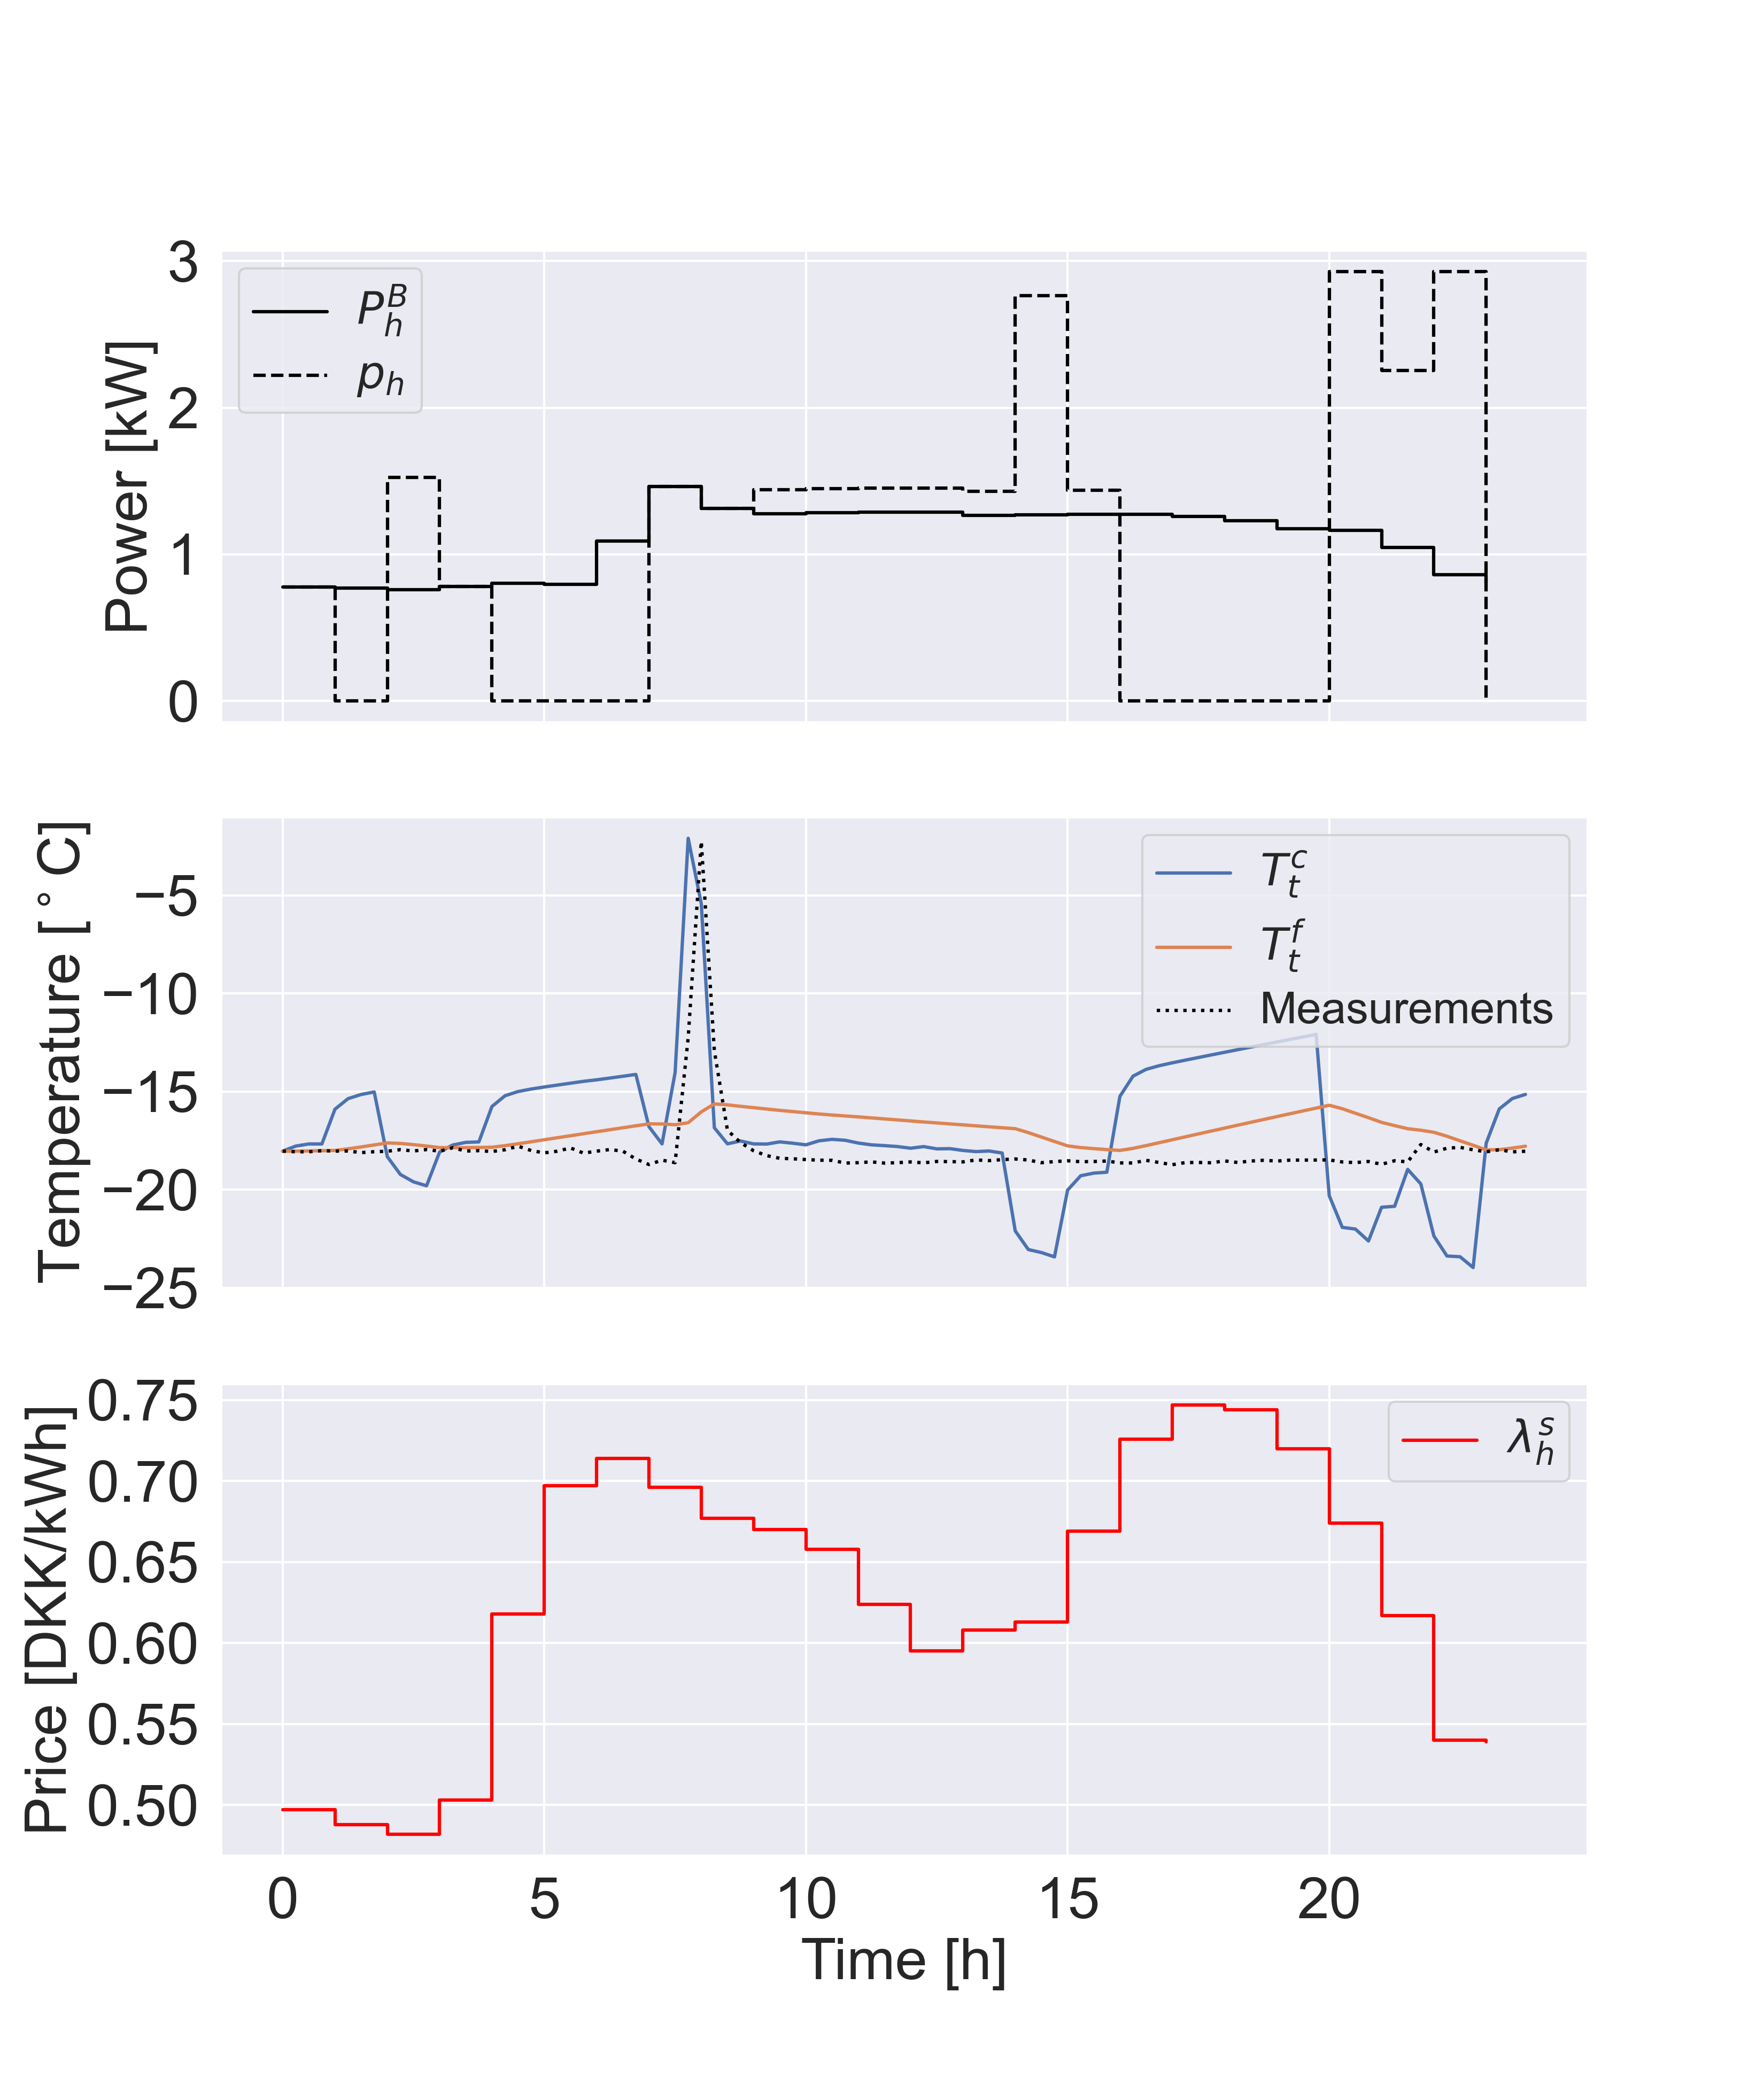
\includegraphics[width=\columnwidth]{../figures/spot_single_case.png}%
        \label{fig_first_case}}
    \hfil
    \subfloat[]{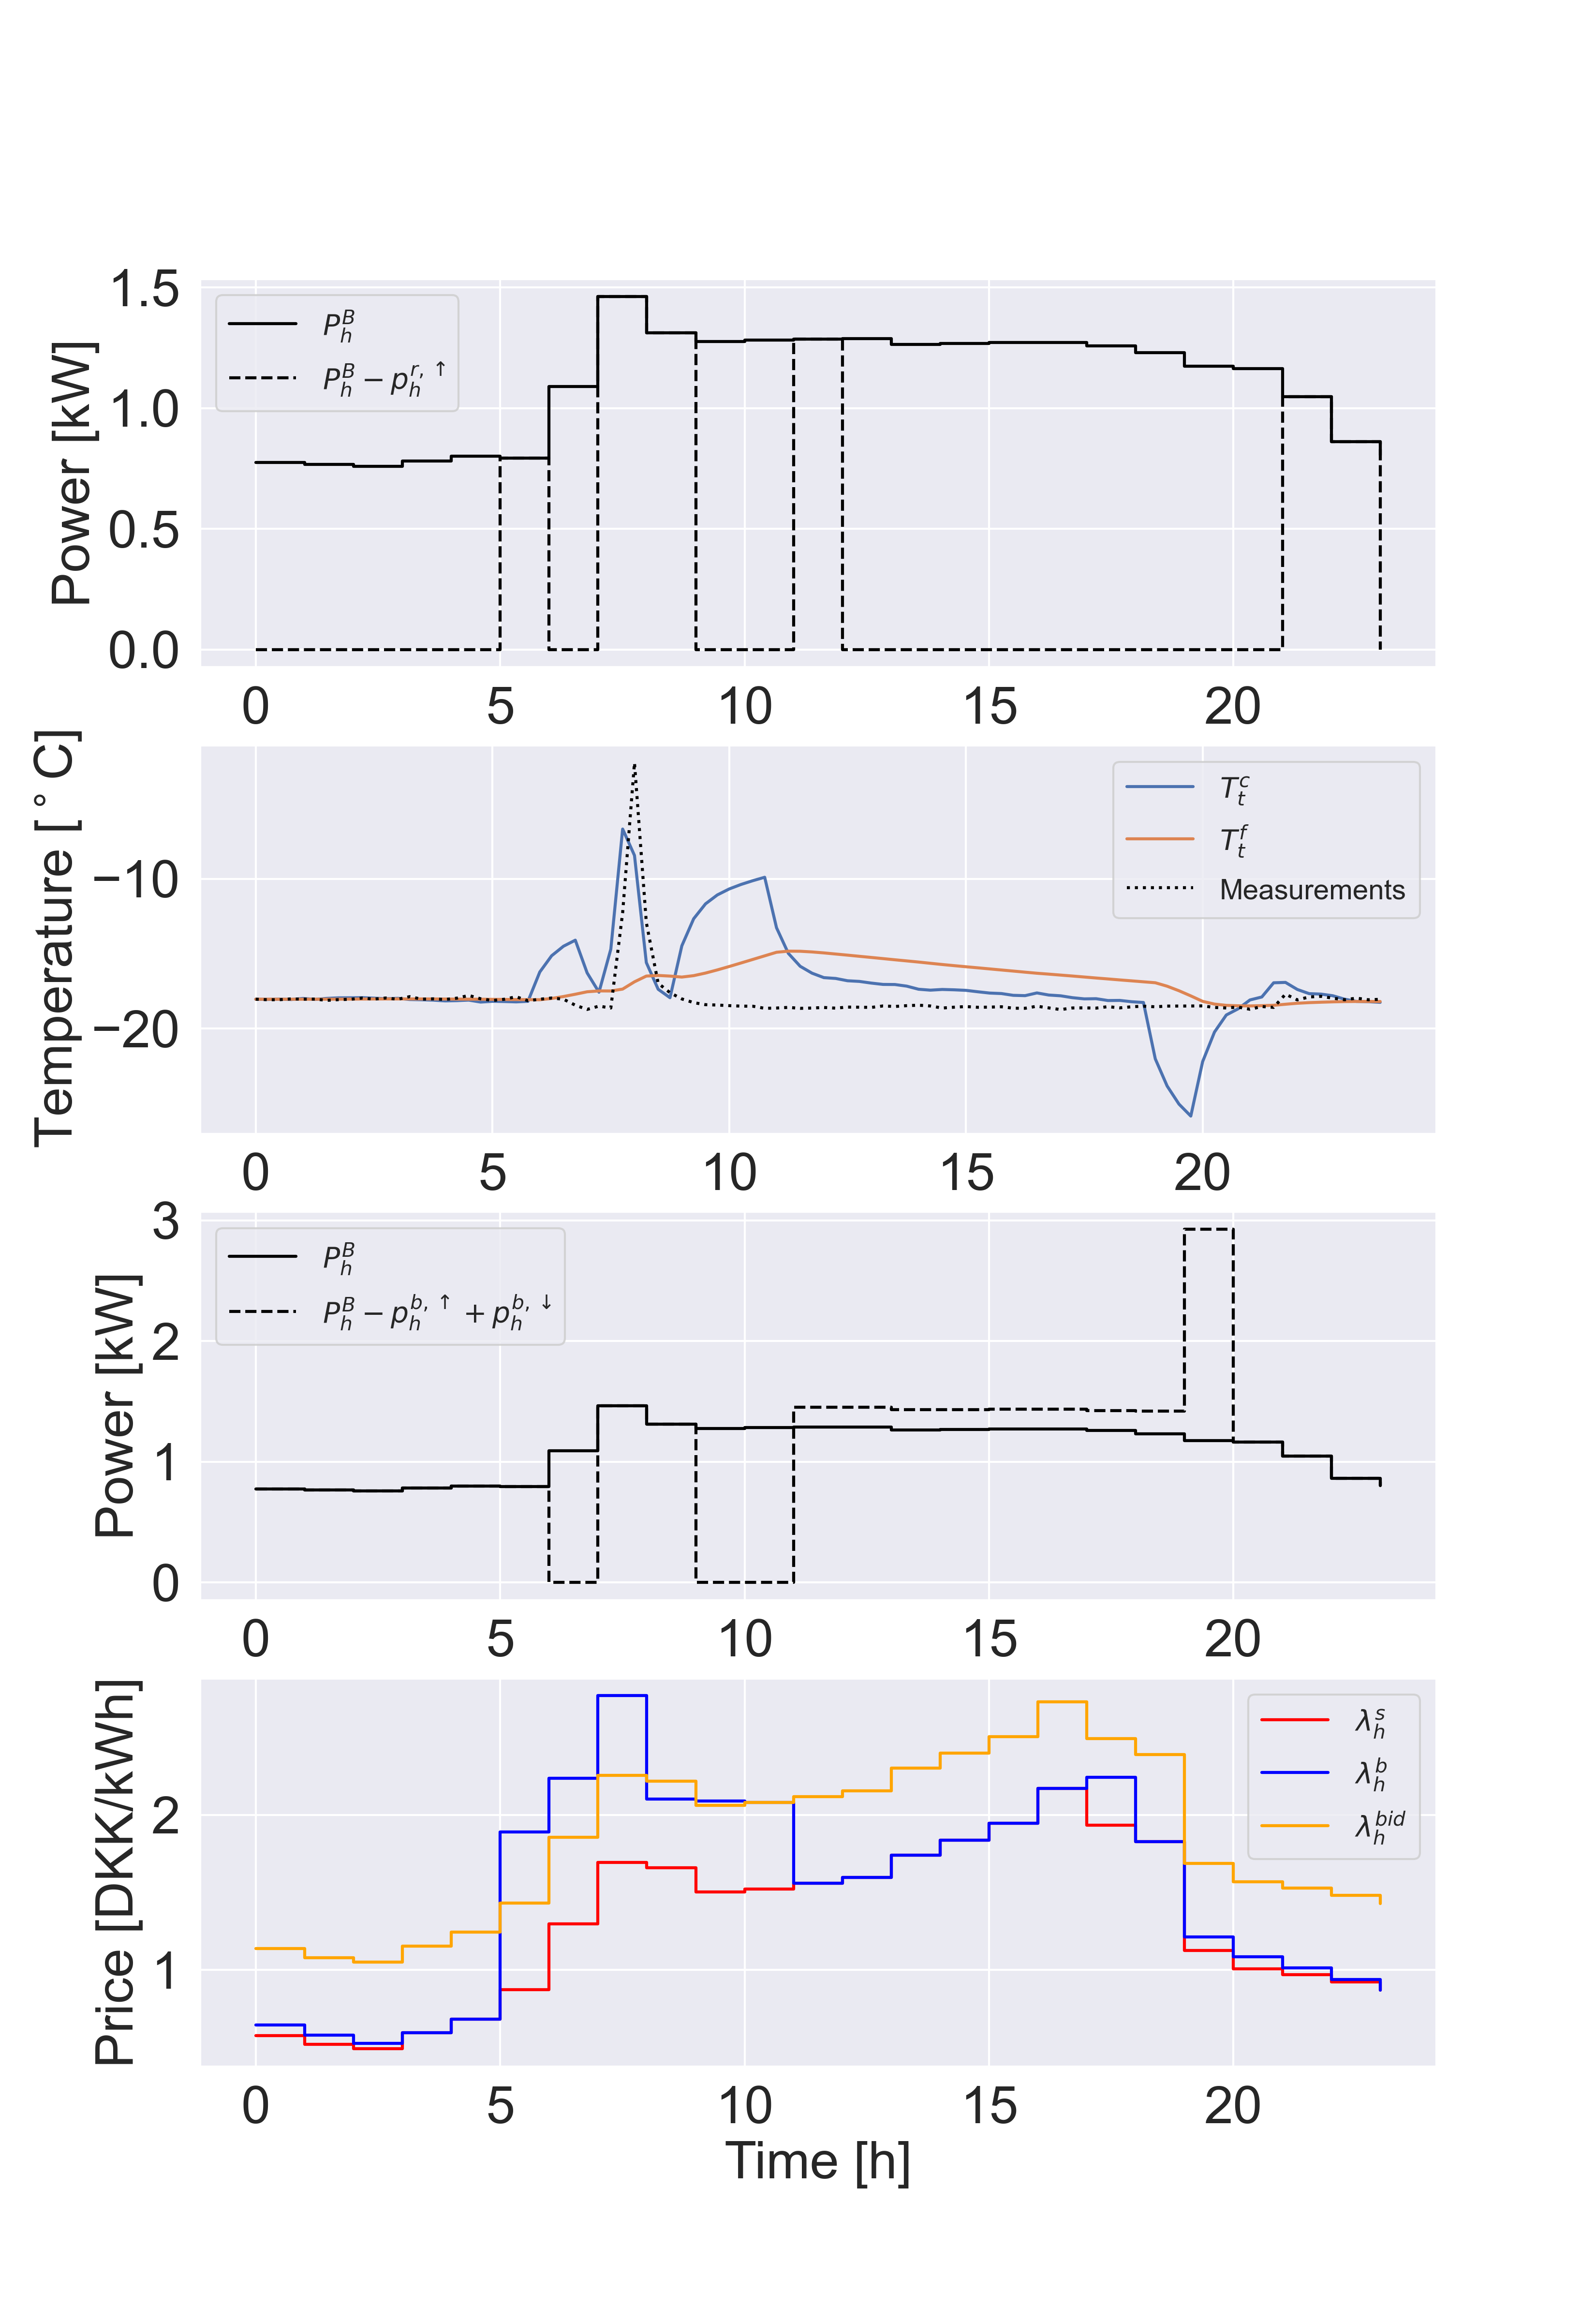
\includegraphics[width=\columnwidth]{../figures/mFRR_single_case.png}%
        \label{fig_second_case}}
    \caption{Comparison between load shifting and mFRR in one IS scenario. \textbf{a}: \textbf{Top}: Power profile when load shifting and baseline power of freezer. \textbf{Middle}: Air and food temperature dynamics. \textbf{Bottom}: Spot price in scenario. \textbf{b}: \textbf{Top}: Reservation capacities and baseline power of freezer. \textbf{Upper middle}: Air and food temperature dynamics. \textbf{Lower Middle}: mFRR activations in this scenarios, i.e., when $\lambda_{h}^{bid} \leq \lambda_{h}^{b}$, $\lambda_{h}^{b} > \lambda_{h}^{s}$ and $p^{r,\uparrow}_{h} > 0$. \textbf{Bottom}: Spot price, balancing price, and bid price in scenario.}
    \label{fig:fig_sim}
\end{figure*}

The results show some interesting features of mFRR and load shifting. Although the savings are higher for load shifting, they are directly proportional to the energy shifted and therefore the temperature deviation in the freezer. For mFRR, this is not the case due to the mechanism of reservation and activation.

Furthermore, settlement costs of the BRP for load shifting were ignored as this reflects the reality of selfish, flexible consumers acting in their own interest. In reality, the BRP would have to pay for the settlement costs or at least buy/sell energy in the intraday market after the day-ahead market clearing and load shifting schedule. But consumers are not necessarily aware of the balance settlement and the electricity market mechanisms. Hence, they have a strong incentive to use their flexibility for load shifting. Some industrial and commercial consumers might not be exposed fully to the spot price, and for those consumers, load shifting is less profitable, but they will still have an incentive to change their deal with the retailer to get full exposure.

For mFRR, it was implicitly assumed that all revenue from reservation and payments go to the flexible consumer. But this neglect the fact that the BRP requires a share of the revenue. Furthermore, there might be an aggregator or technology provider facilitating the aggregation and communication of the flexibility. In this case, the they would also want a share of the revenue. This can potentially reduce the revenue of the consumer significantly and is one of the main challenges of achieving widespread penetration of demand-side flexibility \cite{gade2022ecosystem}.

As mentioned, a single freezer or supermarket must be part of a larger portfolio through an aggregator in order to participate in mFRR. Such an aggregated portfolio has some issues that are neglected here, such as baseline estimation for verification of the demand response, allocation of profits within the portfolio, and accurate capacity estimation of the whole portfolio that bid into mFRR.

Furthermore, mFRR is changing from a 60-min market to a 15-min market in the next few years \cite{MARI}. This makes it more feasible for TCLs to participate given their sensitivity to large temperature deviations.

Nevertheless, load shifting seems more appealing for a flexible consumer compared to mFRR from a monetary point of view. This finding illustrates the importance of designing attractive markets for mFRR if demand-side flexibility is to be used more widely, and perhaps also to disincentivize load shifting for flexible consumers as it could lead to system imbalances.


\subsection{ADMM}

Figure \ref{fig:admm_vs_normal_solution} shows the ADMM convergence to the optimal solution for five scenarios for different step sizes. For most step sizes, it converges quickly but never quite reaches the optimal solution. This is mainly because the algorithm has to achieve consensus on three variables, $p_{h,\omega}^{r,\uparrow}$, $\alpha_{\omega}$, and $\beta_{\omega}$. Experiments showed that it was converging much closer to the optimal solution when removing $\alpha_{\omega}$, and $\beta_{\omega}$.

A large step size emphasizes the need to reach consensus whereas a small step size prioritizes the objective function in (\ref{P1:eq1}). Here, it seems a step size of $\gamma \geq 1$ is more stable and converges quickly.

\begin{figure}[!t]
    \centering
    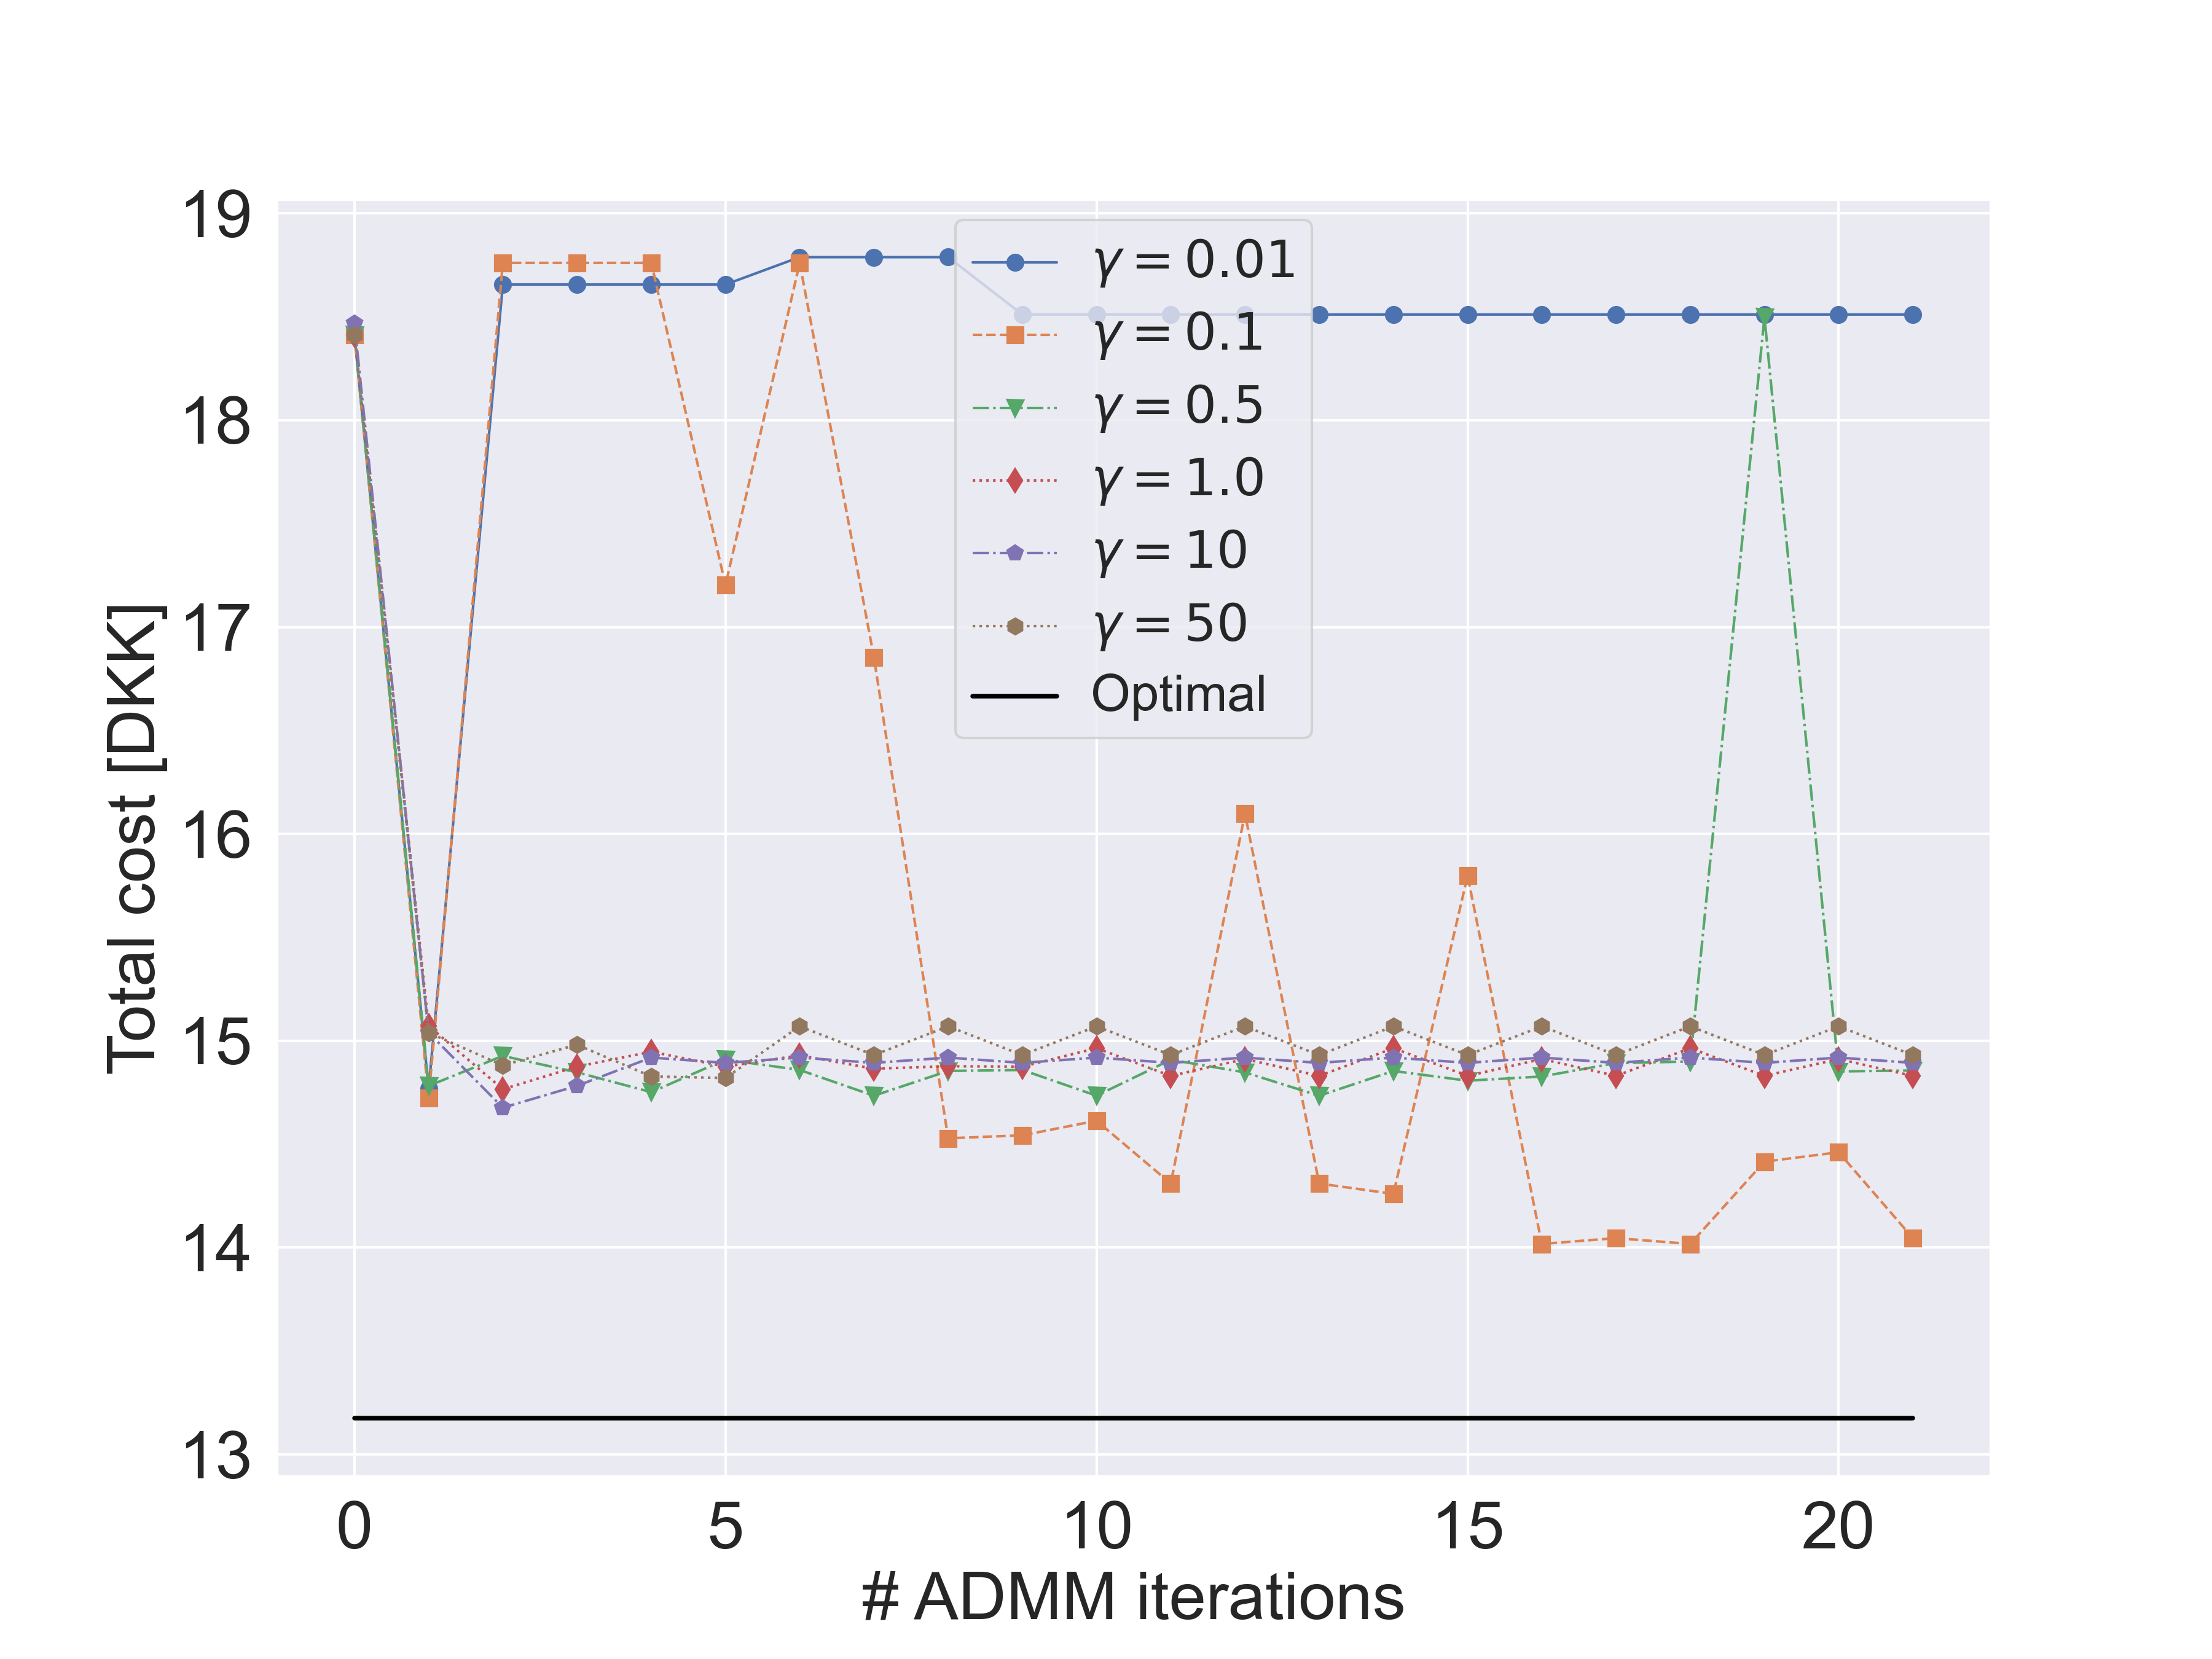
\includegraphics[width=\columnwidth]{../figures/admm_vs_normal_solution.png}
    \caption{ADMM solution versus the optimal solution for five scenarios for different step sizes in the ADMM algorithm.}
    \label{fig:admm_vs_normal_solution}
\end{figure}

Figure \ref{fig:admm_nb_scenarios_effect} shows the effect of including more scenarios in Problem (\ref{P1:compact_model}) using ADMM to solve it. For IS, good solutions are already obtained with 5-10 scenarios, and the same applies for OOS although it seems using 250 scenarios also performs well.

The plot highlights the importance of choosing representative scenarios, especially balancing prices as they determine how much activation is needed, and therefore the bid policy.

\begin{figure}[!t]
    \centering
    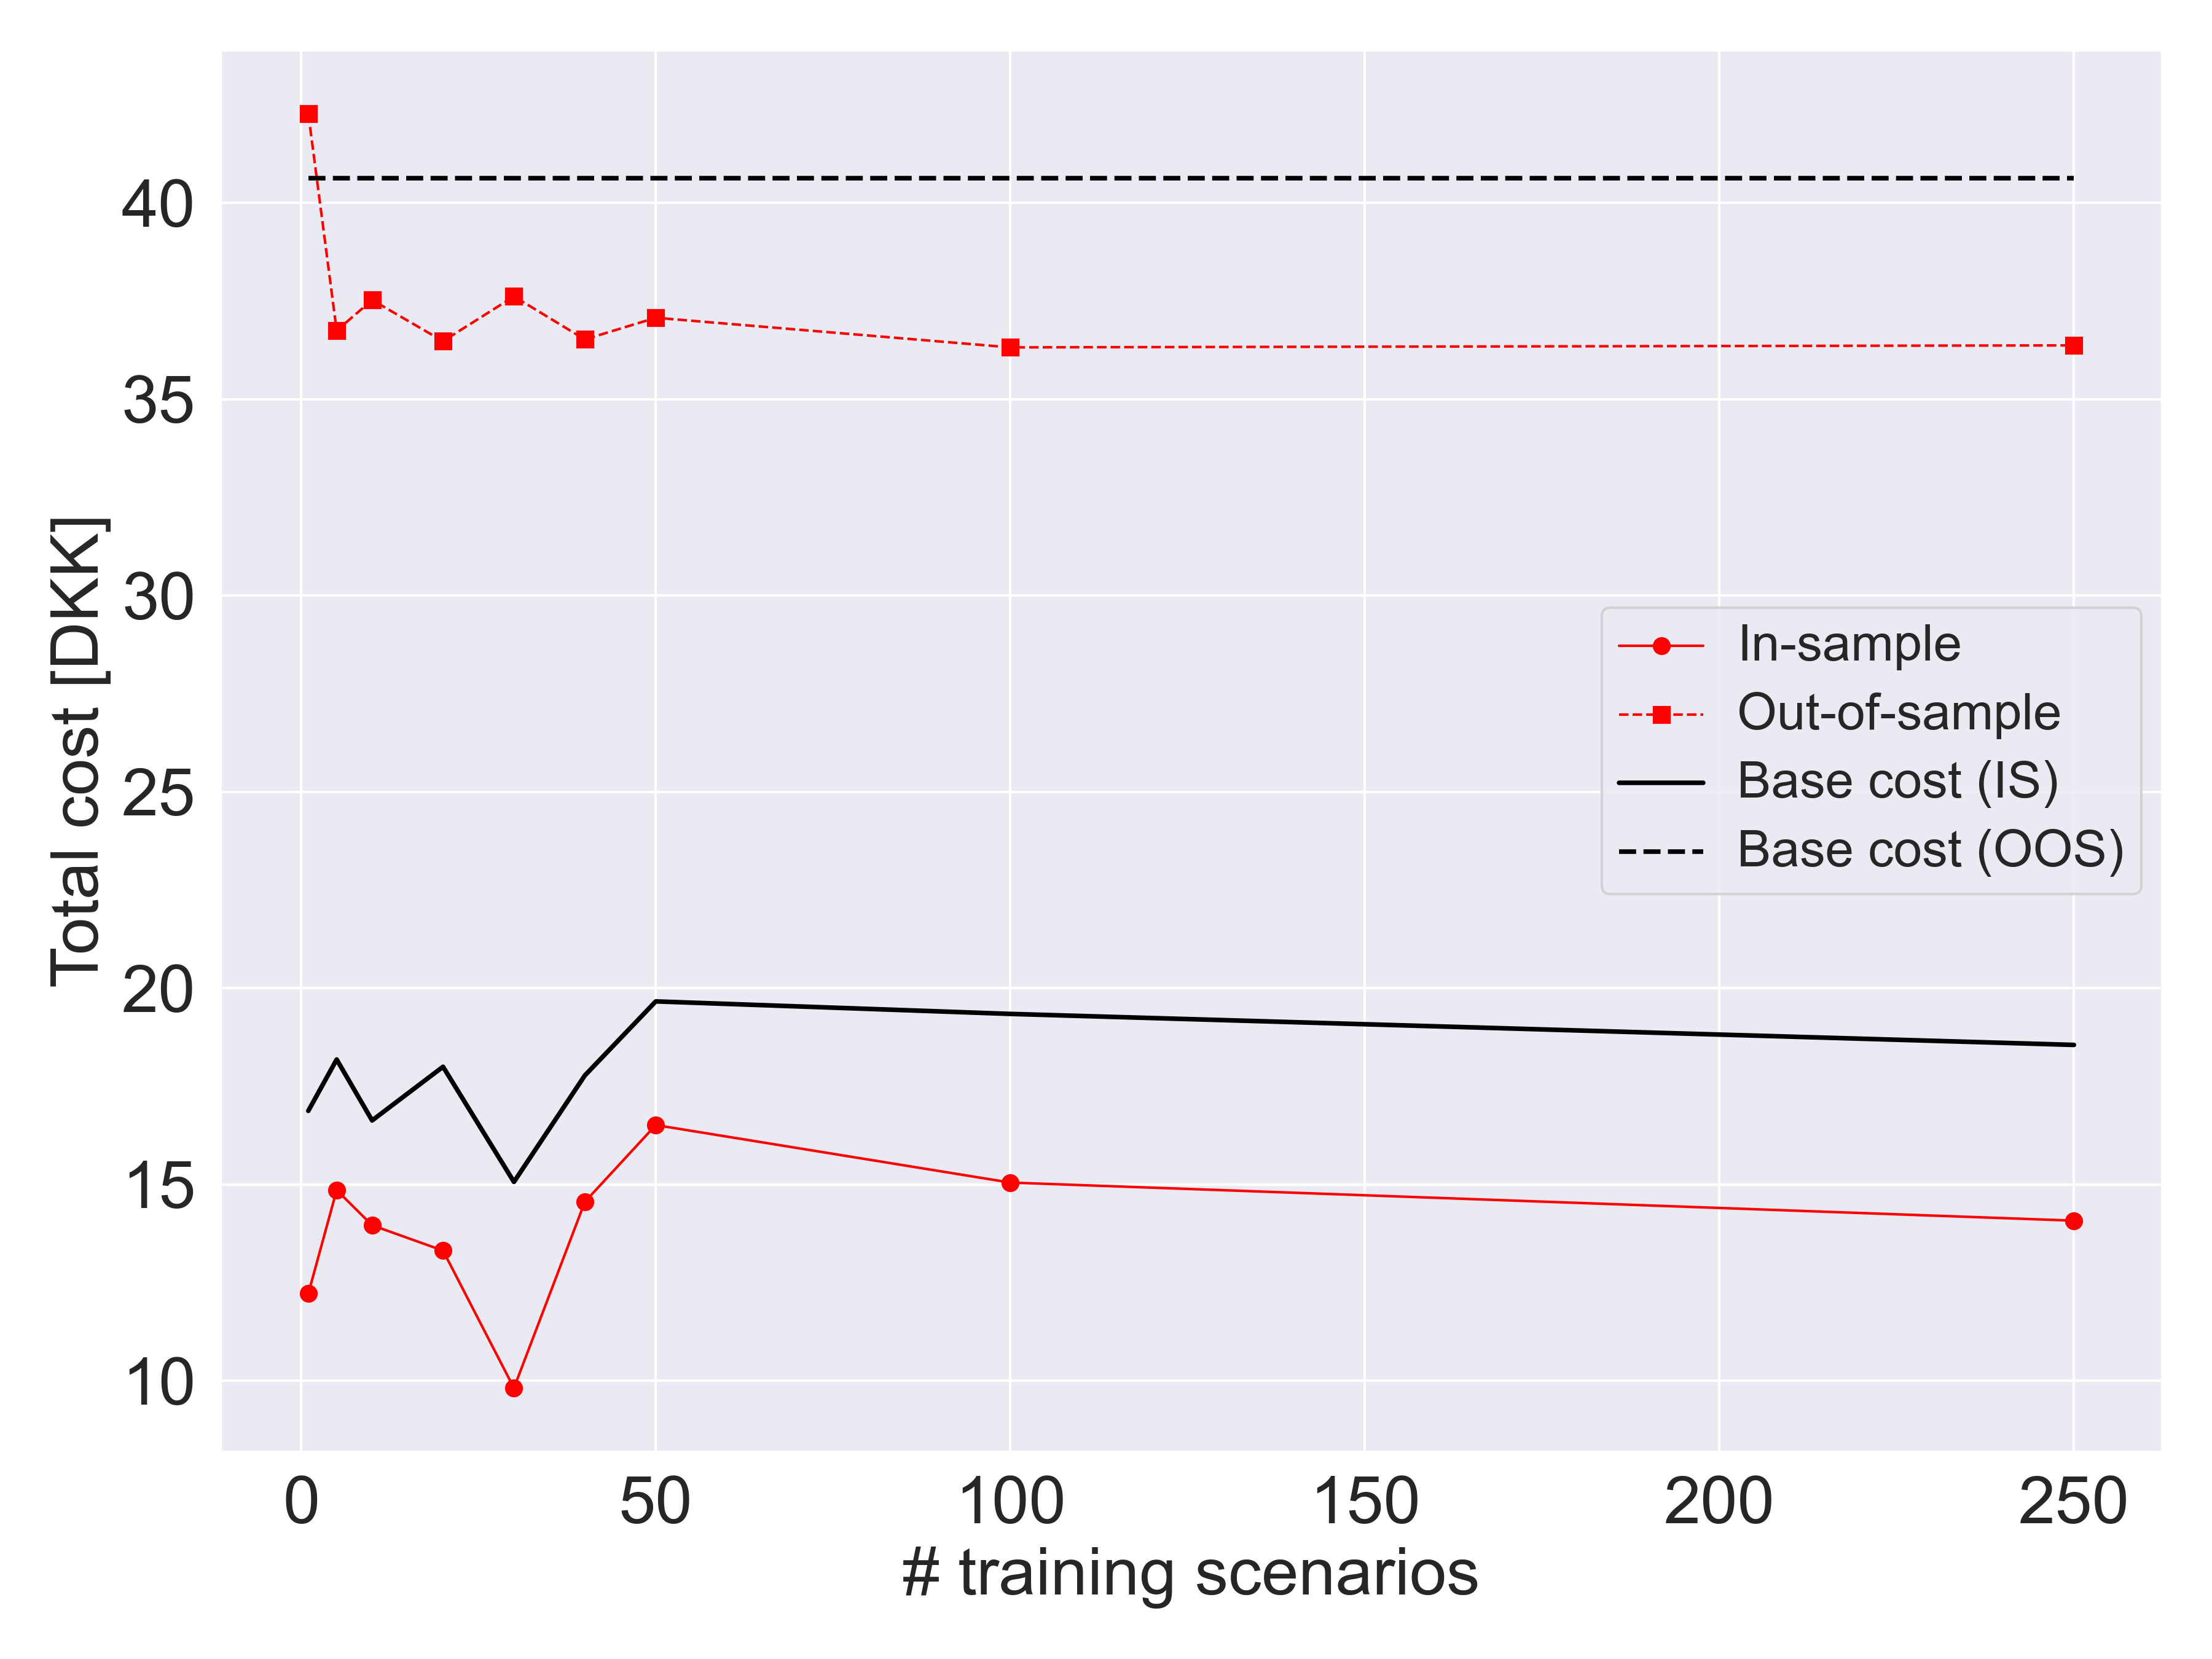
\includegraphics[width=\columnwidth]{../figures/admm_nb_scenarios_effect.png}
    \caption{Effect of number of IS scenarios on OOS performance for ADMM. Both are compared to the baseline costs of the freezer.}
    \label{fig:admm_nb_scenarios_effect}
\end{figure}

% \subsection{Lookback}

% TODO: create plot of effect of lookback parameter.


\vspace{-2mm}
\section{Conclusion}\label{sec:conclusion}
%
We investigated how a supermarket freezer can provide flexibility for mFRR and load shifting in Denmark, and explored which one provides a greater monetary incentive for a flexible load. To this end, we used actual data  from a Danish supermarket. This was done by developing a second-order grey-box model of the temperature dynamics in the freezer with the food temperature as a latent state. In the state-space form, the model was directly incorporated as constraints into a two-stage stochastic MILP problem, whose objective is to maximize the monetary value from the freezer's flexibility. Two scenario generation strategies were implemented: one with a five-day lookback strategy on the spot and balancing market prices in DK2, and the other one  based on price data for those markets in 2021. For mFRR, we used a linear policy, and then linearized the conditions for activation via the McCormick relaxation method. For computational ease, we used an ADMM-based scenario decomposition technique.  An out-of-sample evaluation was done on unseen 2022 price data. We observed that load shifting is more profitable, but has a greater impact on the air and food temperatures in the freezer as opposed to mFRR that depends on the system state and bid price for activation.

We made a set of simplifications and assumptions, whose impacts need to be explored for the future work. The revenue share of BRP and aggregator was not considered. This may change our finding that load shifting is more financially appealing to a flexible load. As mentioned earlier, a single freezer or supermarket must be part of a larger portfolio through an aggregator in order to participate in the mFRR market. Such an aggregated portfolio has some issues that are neglected here, such as the baseline estimation for verification of the demand response, allocation of profits within the portfolio, and an accurate capacity estimation of the whole portfolio that bids in the mFRR market. Furthermore, the European mFRR markets will change from a 60-minute resolution to a 15-minute market in the next few years \cite{MARI}. This makes it more feasible for TCLs to participate in the mFRR market, given their sensitivity to large temperature deviations, and the fact that TCLs can get a passive income when there is no up-regulation need in the power grid.


% {\appendices

\section*{Appendix: Final model formulation}\label{appendix:A}
% \addcontentsline{toc}{section}{Appendices}
% \renewcommand{\thesubsection}{\Alph{subsection}}
% \subsection{Appendix}\label{appendix:A}

%\subsection{Final model formulation}\label{sec:final_model}

% Describe objective function for mFRR and load shifting.

% The set, $\Psi$, then contains all the optimization variables:

% \begin{align}\label{set:OptVariables}
%     \Psi = \{p_{h,\omega}, p^{r, \uparrow}_{h}, & s_{h,\omega}, p^{b, \uparrow}_{h,\omega}, p^{b, \downarrow}_{h,\omega}, u^{\uparrow}_{h,\omega}, y^{\uparrow}_{h,\omega}, z^{\uparrow}_{h,\omega}, u^{\downarrow}_{h,\omega}, y^{\downarrow}_{h,\omega}, z^{\downarrow}_{h,\omega}, \notag \\ & T^{f}_{\omega, t}, T^{c}_{\omega, t}, T^{f,B}_{t}, T^{c, B}_{t}, \lambda_{h}^{bid}, \phi_{h,\omega}, g_{h,\omega}, \Delta \}
% \end{align}


\begingroup
\allowdisplaybreaks

The final optimization model is a two-stage stochastic MILP and is described in full detail in (\ref{FinalModel}) with subsequent explanations.
% First, the objective function is presented. Then all auxillary variables and constraints are presented. Third, constraints related to the power consumption for the freezer is shown. Fourth, the physical constraints for the temperatures are presented. Lastly, the rebound constraints are presented.


% \subsubsection{Objective function}\label{sec:objective_function}


\begin{subequations}\label{P2:FinalModel}
    \begin{align}
        % & \underbrace{C(\text{cost})}_{\text{mFRR}} = - \underbrace{\sum_{h=1}^{24}
        \underset{p^{\rm{r}_{h},\uparrow}, \lambda_{h,\omega}^{\text{bid}},\Gamma_{\omega}}{\textrm{max}} & \quad - \underbrace{\sum_{h=1}^{24} \lambda^{\rm{s}}_{h}P^{\text{Base}}_{h}}_{\textrm{Energy cost}} + \underbrace{\sum_{h=1}^{24}\lambda_{h}^{\rm{r}} p^{\rm{r}, \uparrow}_{h}}_{\textrm{Reservation payment}} +  \notag                                                                                                                                                          \\ \sum_{\omega=1}^{|\Omega|} \pi_{\omega} & \Bigl( \underbrace{\sum_{h=1}^{24}  \lambda_{h,\omega}^{\rm{b}} p^{\rm{b},\uparrow}_{h,\omega}}_{\textrm{Activation payment}} - \underbrace{\sum_{h=1}^{24}  \lambda_{h,\omega}^{\rm{b}} p^{\rm{b},\downarrow}_{h,\omega}}_{\textrm{Rebound cost}} - \underbrace{ \sum_{h=1}^{24}  \lambda^{\rm{p}}s_{h,\omega}}_{\textrm{Penalty cost}} \Bigr) \label{P2:1} \\
        \text{s.t.}
        \quad                                                                                             & \quad \text{State-space model } (\ref{eq:2ndFreezerStateSpace}), \quad \forall{h,\omega} \label{P2:2}                                                                                                                                                                                                                                                                             \\
        \quad                                                                                             & \quad \lambda_{h,\omega}^{\textrm{bid}} = (\ref{eq:affine_policy}),  \label{P2:3}                                                                                                                                                                                                                                                                                                 \\
        \quad                                                                                             & \quad (\ref{eq:bid_constraint_relaxed}), \quad  \label{P2:5}                                                                                                                                                                                                                                                                                                                      \\
        \quad                                                                                             & \quad p_{h,\omega} = P^{\text{Base}}_{h} - p^{b, \uparrow}_{h,\omega} + p^{b, \downarrow}_{h,\omega}, \quad                                                                                                  \forall{h,\omega}                                                                             \label{power:6}                                                        \\
        \quad                                                                                             & \quad p^{r, \uparrow}_h \leq P^{\text{Base}}_h,
        \quad                                                                                                                                                        \forall{h}                                                                                     \label{power:7}                                                                                                                                                                                                           \\
        \quad                                                                                             & \quad p^{b, \uparrow}_{h,\omega} \leq p^{r, \uparrow}_h \mathbbm{1}_{h,\omega}^{\lambda^{b}_{h,\omega} > \lambda^{\rm{s}}_{h}} , \quad                                                                            \forall{h,\omega}                                                                             \label{power:8}                                                   \\
        \quad                                                                                             & \quad p^{b, \uparrow}_{h,\omega} \leq u_{h,\omega}^{\uparrow} (P^{\text{Base}}_{h} - P^{\text{Min}}) , \quad                                                                                                       \forall{h,\omega}                                                                             \label{power:9}                                                  \\
        \quad                                                                                             & \quad p^{b, \downarrow}_{h,\omega} \leq u^{\downarrow}_{h,\omega} (P^{\text{Nom}} -P^{\text{Base}}_{h}), \quad                                                                                              \forall{h,\omega}                                                                             \label{power:10}                                                        \\
        \quad                                                                                             & \quad P^{\text{Min}} \leq p_{h,\omega} \leq P^{\text{Nom}}, \quad                                                                                                                                           \forall{h,\omega}                                                                             \label{power:11}                                                        \\
        \quad                                                                                             & \quad 0 \leq s_{h,\omega} \leq P^{\text{Base}}_{h}, \quad                                                                                                                                                   \forall{h,\omega}                                                                             \label{power:12}                                                        \\
        % \quad                                                                                             & \quad p^{b, \uparrow}_{h,\omega} + s_{h,\omega} \geq p^{r,\uparrow}_{h} \cdot \mathbbm{1}_{h,\omega}^{(\lambda^{\text{bid}}_{h} < \lambda^{b}_{h,\omega}, \lambda^{b}_{h,\omega} > \lambda^{s}_{h})}, \quad                                                                                                              \forall{h,\omega} \label{power:13} \\
        \quad                                                                                             & \quad p^{b, \downarrow}_{h,\omega} \geq 0.10 \cdot u^{\downarrow}_{h,\omega} (P^{\text{Nom}} - P^{\text{Base}}_{h}), \quad                                                                                  \forall{h,\omega}                                                                             \label{power:14}                                                        \\
        \quad                                                                                             & \quad p^{r, \uparrow}_{h} \leq P^{\text{Base}}_{h} (1 - \mathbbm{1}_{h}^{\text{df}}), \quad                                                                                                                 \forall{h} \label{power:15}                                                                                                                                           \\
        \quad                                                                                             & \quad u_{h-1,\omega}^{\uparrow} - u_{h,\omega}^{\uparrow} + y_{h,\omega}^{\uparrow} - z_{h,\omega}^{\uparrow} = 0, \notag                                                                                                                                                                                                                                                         \\ \quad & \quad           \forall{\omega}, \forall{h} = \{2 \ldots 24 \}                                                                                                                                        \label{aux:1}                                       \\
        \quad                                                                                             & \quad y_{h,\omega}^{\uparrow} + z_{h,\omega}^{\uparrow} \leq 1 \quad                                                             \forall{h,\omega}                                                                                                                                                                     \label{aux:2}                                              \\
        \quad                                                                                             & \quad u_{h-1,\omega}^{\downarrow} - u_{h,\omega}^{\downarrow} + y_{h,\omega}^{\downarrow} - z_{h,\omega}^{\downarrow} = 0, \notag                                                                                                                                                                                                                                                 \\ \quad & \quad   \forall{\omega}, \forall{h} = \{2 \ldots 24 \}                                                                                                                                        \label{aux:3}                                       \\
        \quad                                                                                             & \quad y_{h,\omega}^{\downarrow} + z_{h,\omega}^{\downarrow} \leq 1 \quad                                                         \forall{h,\omega}                                                                                                                                                                     \label{aux:4}                                              \\
        \quad                                                                                             & \quad u_{h,\omega}^{\uparrow} + u_{h,\omega}^{\downarrow} \leq 1 \quad                                                           \forall{h,\omega}                                                                                                                                                                     \label{aux:5}                                              \\
        \quad                                                                                             & \quad y_{h,\omega}^{\uparrow} + y_{h,\omega}^{\downarrow} \leq 1 \quad                                                           \forall{h,\omega}                                                                                                                                                                     \label{aux:6}                                              \\
        \quad                                                                                             & \quad z_{h,\omega}^{\uparrow} + z_{h,\omega}^{\downarrow} \leq 1 \quad                                                           \forall{h,\omega} \label{aux:7}                                                                                                                                                                                                                  \\
        \quad                                                                                             & \quad T^{\rm{f}}_{J,\omega} \leq T^{f, \text{Base}}_{J}, \quad \forall{\omega} \label{temp:1}                                                                                                                                                                                                                                                                                     \\
        \quad                                                                                             & \quad T^{\rm{c},\text{Base}}_{t} - \Delta \leq T^{\rm{c}}_{t, \omega}, \quad                                                                                                                                                                                                                                                                    \forall{t, \omega} \label{temp:2} \\
        \quad                                                                                             & \quad T^{\rm{c},\text{Base}}_{t} - \Delta \geq T^{\rm{c}}_{t, \omega}, \quad                                                                                                                                                                                                                                                                    \forall{t, \omega} \label{temp:3} \\
        \quad                                                                                             & \quad \Delta \leq \Delta^{\text{max}} \label{temp:4}                                                                                                                                                                                                                                                                                                                              \\
        \quad                                                                                             & \quad y^{\downarrow}_{h, \omega} \geq z^{\uparrow}_{h, \omega}, \quad                                                                                                                                                                                                                                                                 \forall{h, \omega} \label{rebound:1}        \\
        \quad                                                                                             & \quad y^{\downarrow}_{h, \omega} \leq z^{\uparrow}_{h, \omega}, \quad                                                                                                                                                                                                                                                                 \forall{h, \omega} \label{rebound:2}        \\
        \quad                                                                                             & \quad \sum_{t=4\cdot(h-1)}^{4 h} T^{\rm{f}}_{t, \omega} - T^{\rm{f}, \text{Base}}_{t} \geq - (1 - z^{\downarrow}_{h, \omega}) \cdot M, \notag                                                                                                                                                                                                                                     \\ \quad & \quad  \forall{\omega}, \forall{h} \label{rebound:3}                                                                                                                                                                                 \\
        \quad                                                                                             & \quad \sum_{t=4\cdot(h-1)}^{4 h} T^{\rm{f}}_{t, \omega} - T^{\rm{f}, \text{Base}}_{t} \leq - (1 - z^{\downarrow}_{h, \omega}) \cdot M, \notag                                                                                                                                                                                                                                     \\ \quad & \quad  \forall{\omega}, \forall{h} \label{rebound:4}                                                                                                                                                                                 \\
        \quad                                                                                             & \quad \sum_{k=0}^{h} y^{\downarrow}_{\omega, k} \leq y^{\uparrow}_{\omega, k}, \quad \forall{h, \omega} \label{up_reg_first}                                                                                                                                                                                                                                                      \\
        \quad                                                                                             & \quad \Bigl( \bm{p}^{\rm{r},\uparrow}, \bm{\lambda}_{\omega}^{\text{bid}}, \bm{p}_{\omega}^{\rm{b},\uparrow}, \bm{p}_{\omega}^{\rm{b},\downarrow}, \bm{s}_{\omega}, \bm{T}_{\omega}^{\rm{c}}, \bm{T}_{\omega}^{\rm{f}}, \notag                                                                                                                                                    \\ \quad & \quad \bm{T}_{\omega}^{\rm{c,B}}, \bm{T}_{\omega}^{\rm{f,B}}, \bm{\phi}_{\omega}, \bm{g}_{\omega} \Bigr) \in \mathbb{R}^{n}  \label{P2:cont}
        \\
        \quad                                                                                             & \quad \bm{u}_{\omega}, \bm{z}_{\omega}, \bm{y}_{\omega} \in \{0,1\},  \label{P2:binary}
    \end{align}
\end{subequations}

The objective function in (\ref{P2:1}) maximized revenue from mFRR while reducing the rebound and penalty cost for all equiprobable scenarios.

Equation (\ref{P2:2}) is the state-space model for the temperature dynamics. Furthermore, there is a set of identical constraints to (\ref{P2:2}) that simulate the baseline temperatures, $T^{\rm{f},\rm{B}}_{t}$ and $T^{\rm{c},\rm{B}}_{t}$, using the baseline power, $P^{\text{Base}}_{h}$.. Note, the freezer specific variables are indexed by $t$, representing a time step $dt = 0.25$ whereas all other variables are indexed by hour $h$.

Equations (\ref{P2:3}-\ref{P2:5}) are the bidding policy.

Equations (\ref{power:6}-\ref{power:12}) encode the power consumption constraints.

Equations (\ref{aux:1}-\ref{aux:7}) define the behavior for the six binary auxiliary variables to identify transitions from/to up-regulation and down-regulation (see \cite{morales2013integrating} for details).

Equations (\ref{temp:1}-\ref{temp:4}) control the maximum temperature deviation and end temperature.

Equations (\ref{rebound:1}-\ref{rebound:4}) control the rebound behavior such that the rebound finishes when the temperature is below the baseline temperature. Note, $M$ is a sufficiently big number such that the food temperature is allowed to deviate from the baseline. Also, they ensure that the rebound happens right after up-regulation.

lastly, equation (\ref{up_reg_first}) ensures that up-regulation happens first. This makes sense since it is not possible (or at least difficult) to anticipate potential up-regulation events in the power grid. As such, it does not make sense to pre-cool (or pre-heat) a TCL in the context of mFRR.

% \subsubsection{Auxillary variables and constraints}\label{sec:aux_constraints}

% First, we describe the necessary auxillary variables and constraints to identify when up- and down-regulation occurs compared to the baseline power, $P^{\text{Base}}_{h}$. This is required since the costs and revenues from up-regulation and rebound must be determined explicitly. We therefore introduce the following six binary variables \cite{morales2013integrating}:
% \\
% \begin{itemize}
%     \item $u^{\uparrow}_{h,\omega} \in \{0,1\}$ equal to 1 when starting to deliver up-regulation
%     \item $y^{\uparrow}_{h,\omega} \in \{0,1\}$ equal to 1 during up-regulation
%     \item $z^{\uparrow}_{h,\omega} \in \{0,1\}$ equal to 1 when to stopping up-regulation
%     \item $u^{\downarrow}_{h,\omega} \in \{0,1\}$ equal to 1 when starting to deliver down-regulation
%     \item $y^{\downarrow}_{h,\omega} \in \{0,1\}$ equal to 1 during down-regulation
%     \item $z^{\downarrow}_{h,\omega} \in \{0,1\}$ equal to 1 when to stopping down-regulation
% \end{itemize}

% \noindent The following constraints implements the logic:

% \begin{subequations}\label{eq:auxillary_constraints}
%     \begin{align}
%         u_{h-1,\omega}^{\uparrow} - u_{h,\omega}^{\uparrow} + y_{h,\omega}^{\uparrow} - z_{h,\omega}^{\uparrow} = 0 \quad         & \forall{\omega}, \forall{h} = \{2 \ldots 24 \} \\
%         y_{h,\omega}^{\uparrow} + z_{h,\omega}^{\uparrow} \leq 1 \quad                                                            & \forall{h,\omega}                              \\
%         u_{h-1,\omega}^{\downarrow} - u_{h,\omega}^{\downarrow} + y_{h,\omega}^{\downarrow} - z_{h,\omega}^{\downarrow} = 0 \quad & \forall{\omega}, \forall{h} = \{2 \ldots 24 \} \\
%         y_{h,\omega}^{\downarrow} + z_{h,\omega}^{\downarrow} \leq 1 \quad                                                        & \forall{h,\omega}                              \\
%         u_{h,\omega}^{\uparrow} + u_{h,\omega}^{\downarrow} \leq 1 \quad                                                          & \forall{h,\omega}                              \\
%         y_{h,\omega}^{\uparrow} + y_{h,\omega}^{\downarrow} \leq 1 \quad                                                          & \forall{h,\omega}                              \\
%         z_{h,\omega}^{\uparrow} + z_{h,\omega}^{\downarrow} \leq 1 \quad                                                          & \forall{h,\omega}
%     \end{align}
% \end{subequations}

% \subsubsection{Power constraints}\label{sec:power_constraints}

% The power consumption of the freezer is constrained by:

% \begin{subequations}\label{eq:power_constraints}
%     \begin{align}
%         p_{h,\omega} = P^{\text{Base}}_{h} - p^{b, \uparrow}_{h,\omega} + p^{b, \downarrow}_{h,\omega}, \quad                                                                                                 & \forall{h,\omega}                                                                             \label{con_power:subeq1}  \\
%         p^{r, \uparrow}_h \leq P^{\text{Base}}_h, \quad                                                                                                                                                       & \forall{h}                                                                                     \label{con_power:subeq2} \\
%         p^{b, \uparrow}_{h,\omega} \leq p^{r, \uparrow}_h \mathbbm{1}_{h,\omega}^{\lambda^{b}_{h,\omega} > \lambda^{s}_{h}} , \quad                                                                           & \forall{h,\omega}                                                                             \label{con_power:subeq3}  \\
%         p^{b, \uparrow}_{h,\omega} \leq u_{h,\omega}^{\uparrow} (P^{\text{Base}}_{h} - P^{Min}) , \quad                                                                                                       & \forall{h,\omega}                                                                             \label{con_power:subeq4}  \\
%         p^{b, \downarrow}_{h,\omega} \leq u^{\downarrow}_{h,\omega} (P^{\text{Nom}} -P^{\text{Base}}_{h}), \quad                                                                                              & \forall{h,\omega}                                                                             \label{con_power:subeq5}  \\
%         P^{\text{Min}} \leq p_{h,\omega} \leq P^{\text{Nom}}, \quad                                                                                                                                           & \forall{h,\omega}                                                                             \label{con_power:subeq6}  \\
%         0 \leq s_{h,\omega} \leq P^{\text{Base}}_{h}, \quad                                                                                                                                                   & \forall{h,\omega}                                                                             \label{con_power:subeq7}  \\
%         p^{b, \uparrow}_{h,\omega} + s_{h,\omega} \geq p^{r,\uparrow}_{h} \cdot \mathbbm{1}_{h,\omega}^{(\lambda^{\text{bid}}_{h} < \lambda^{b}_{h,\omega}, \lambda^{b}_{h,\omega} > \lambda^{s}_{h})}, \quad & \forall{h,\omega} \label{con_power:subeq8}                                                                              \\
%         p^{b, \downarrow}_{h,\omega} \geq 0.10 \cdot u^{\downarrow}_{h,\omega} (P^{\text{Nom}} - P^{\text{Base}}_{h}), \quad                                                                                  & \forall{h,\omega}                                                                             \label{con_power:subeq9}  \\
%         p^{r, \uparrow}_{h} \leq P^{\text{Base}}_{h} (1 - \mathbbm{1}_{h}^{\text{df}}), \quad                                                                                                                 & \forall{h} \label{con_power:subeq10}
%     \end{align}
% \end{subequations}

% Constraint (\ref{con_power:subeq1}) sets the power equal to the baseline power unless there is up- or down-regulation. Constraint (\ref{con_power:subeq2}) bounds the reservation power to the baseline power. Constraint (\ref{con_power:subeq3}) ensures that up-regulation is zero when the system does not need it, and at the same time bounds it to the reservation power. Constraint (\ref{con_power:subeq4}) ensures that up-regulation is 0 whenever $u^{\uparrow}_{h,\omega} = 0$, and otherwise bounded to the maximum power that can be upregulated. Constraint (\ref{con_power:subeq5}) works the same way for down-regulation. Constraint (\ref{con_power:subeq6}) bounds the power to be between the minimum and nominal power. Constraint (\ref{con_power:subeq7}) bounds the slack variable which is the energy not delivered as promised. Constraint (\ref{con_power:subeq8}) is the bi-linear constraint from (\ref{eq:bid_constraint}). Constraint (\ref{con_power:subeq9}) ensures that down-regulation is equal to at least 10\% of the down-regulation capacity. Lastly, constraint (\ref{con_power:subeq10}) prohibits any up-regulation when defrosting occurs.

% \subsubsection{Physical constraints}\label{sec:temperature_constraints}

% The state-space model in (\ref{eq:2ndFreezerStateSpace}) is simply added as constraints with $p_{t,\omega}$ being the power of the freezer and an additional index for each scenario, $\omega$.

% Note, the freezer specific variables are indexed by $t$, representing a time step $dt = 0.25$ whereas all other variables are indexed by hour $h$.

% Furthermore, there is a set of identical constraints to (\ref{eq:2ndFreezerStateSpace}) that simulates the baseline temperatures, $T^{f,B}_{t}$ and $T^{c,B}_{t}$, using the baseline power, $P^{Base}_{h}$. These are used for the following boundary constraint, as well as the rebound constraints in Section \ref{sec:rebound_constraints}.

% \begin{align}\label{eq:boundary_constraint}
%     T^{f}_{96,\omega} \leq T^{f, \text{Base}}_{96}, \quad \forall{\omega}
% \end{align}

% The boundary constraint in (\ref{eq:boundary_constraint}) ensures that the optimization does not exploit the end state.

% Temperature constraints to the air temperature can easily be added to limit the flexibility of the TCL by introducing a maximum temperature difference to the baseline temperature, $\Delta^{\text{max}}$:

% \begin{subequations}\label{eq:delta_max_constraints}
%     \begin{align}
%         T^{c,\text{Base}}_{t} - \Delta \leq T^{c}_{t, \omega}, \quad & \forall{t, \omega} \\
%         T^{c,\text{Base}}_{t} - \Delta \geq T^{c}_{t, \omega}, \quad & \forall{t, \omega} \\
%         \Delta \leq \Delta^{\text{max}}
%     \end{align}
% \end{subequations}

% \subsubsection{Rebound constraints}\label{sec:rebound_constraints}

% The rebound constraints ensures that a rebound happens right after an up-regulation by down-regulating:

% \begin{subequations}\label{eq:rebound_constraints_1}
%     \begin{align}
%         y^{\downarrow}_{h, \omega} \geq z^{\uparrow}_{h, \omega}, \quad & \forall{h, \omega} \\
%         y^{\downarrow}_{h, \omega} \leq z^{\uparrow}_{h, \omega}, \quad & \forall{h, \omega}
%     \end{align}
% \end{subequations}


% Furthermore, the following rebound constraints ensures that the rebound will take place until the food temperature is equal to the baseline food temperature, which can be considered the setpoint food temperature:

% \begin{subequations}\label{eq:rebound_constraints_2}
%     \begin{align}
%         \sum_{t=4\cdot(h-1)}^{4 h} T^{f}_{t, \omega} - T^{f, \text{Base}}_{t} \geq - (1 - z^{\downarrow}_{h, \omega}) \cdot M, \quad & \forall{\omega}, \forall{h} \\
%         \sum_{t=4\cdot(h-1)}^{4 h} T^{f}_{t, \omega} - T^{f, \text{Base}}_{t} \leq - (1 - z^{\downarrow}_{h, \omega}) \cdot M, \quad & \forall{\omega}, \forall{h}
%     \end{align}
% \end{subequations}

% In constraints (\ref{eq:rebound_constraints_2}), $M$ is a sufficiently big number such that the food temperature is allowed to deviate from the baseline.

% Lastly, the following constraint ensures that up-regulation happens before down-regulation:

% \begin{align}\label{eq:up_regulation_first}
%     \sum_{k=0}^{h} y^{\downarrow}_{\omega, k} \leq y^{\uparrow}_{\omega, k}, \quad \forall{h, \omega}
% \end{align}

% This makes sense since it is not possible (or at least difficult) to anticipate potential up-regulation events in the power grid. As such, it does not make sense to pre-cool (or pre-heat) a TCL in the context of mFRR.


\endgroup

% \section*{Appendix A}\label{appendix:A}
% % \addcontentsline{toc}{section}{Appendices}
% % \renewcommand{\thesubsection}{\Alph{subsection}}
% % \subsection{Appendix}\label{appendix:A}

% Hao et al. \cite{hao2014aggregate} describes how a TCL can be modelled as a virtual battery using a first-order thermal-electric ODE:

% \begin{align}\label{eq:hao}
%     \frac{dT(t)}{dt} = \frac{1}{C}\left( \frac{1}{R}(T^{a}(t) - T(t)) + \eta P(t) \right)
% \end{align}

% Here, $T(t)$ is the temperature, $C$ is the thermal capacitance (kWh/$^{\circ}$C), $R$ is the thermal resistance ($^{\circ}$C/kW), $\eta$ is the coefficient of performance (COP), i.e., the cooling/heating effect, $P(t)$ is the power to the TCL, and $T^{a}(t)$ is the ambient temperature outside the TCL (typically around 20 $^{\circ}$C in an indoor environment).

% Note, (\ref{eq:hao}) can readily be formulated in a deterministic, state-space model as in (\ref{eq:sde1}). The following difference equation yields the Euler approximation of (\ref{eq:hao}) which can be used in an optimization model (with the same time step $dt$):

% \begin{align}\label{eq:hao_discretized}
%     T_{t+1} = T_t + dt\cdot \left( \frac{1}{C}\left( \frac{1}{R}(T^{a}_t - T_t) + \eta P_t \right)  \right)
% \end{align}

% Eq. (\ref{eq:hao}) and (\ref{eq:hao_discretized}) constitutes the most simple model of a TCL one can imagine, but, nevertheless, has a quite powerful interpretation: the rate of change of temperature is determined by the heat flux to the surrounding environment and the heat flux from the power source to the TCL. It thus captures the most fundamental temperature dynamics of a TCL.

% The steady-state power in (\ref{eq:hao}) is given by:

% \begin{align}\label{eq:hao_ss}
%     P^{ss}(t) = \frac{T^{a}(t) - T(t)}{\eta R}
% \end{align}

% The steady-state power is thus the power required to keep the temperature of the TCL constant with respect to the outside temperature, $T^{a}(t)$, given the efficiency of the system and the thermal resistance. A better energy efficiency can be achieved by either 1) increasing the mechanical efficiency of the cooling/heating system or 2) increasing the thermal resistance to the outside temperature by, e.g., insulating a freezer.

% The drawback of the first-order model in (\ref{eq:hao}) is that it is only parameterized by three parameters, and it excludes disturbances. Hence, it might not be an accurate model of a real system. The model can easily be extended to include more complicated dynamics such as heat exchange with a barrier between $T^{a}(t)$ and $T(t)$, additional disturbance terms (e.g., when a fridge is opened), hourly values of $C$ and $R$, etc. Nevertheless, (\ref{eq:hao}) serves as a good starting point for a simple TCL model.

% \section*{Appendix B}\label{appendix:B}
% Appendix two text goes here.
}


\section*{Acknowledgement}

The authors would like to acknowledge the financial support from Innovation Fund Denmark under grant number 0153-00205B for partially funding the work in this paper. The authors would also like to thank Christian Ahn Albertsen (IBM Client Innovation Center) for all our discussions and his feedback which has been particularly valuable regarding practical challenges faced for demand-response. The authors would also like to thank Bennevis Crowley (DTU) for reading the paper and providing feedback on corrections, figures, and phrases. The authors would also like to thank the Centre for Utilities and Supply at Energistyrelsen (Danish Energy Agency) for allowing us to present our work to them while also elaborating their perspective on Market Model 3.0 and their intentions.



\bibliographystyle{IEEEtran}
\bibliography{tex/bibliography/Bibliography.bib}

\newpage

\begin{IEEEbiographynophoto}{Peter A.V. Gade}
    is an Industrial PhD researcher at IBM and affiliated with the Technical University of Denmark, Kongens Lyngby, Denmark, in the Energy Markets and Analytics Section within the Power and Energy Systems division at the Wind and Energy Systems Department. His research focuses on demand-side flexibility and the revenue streams from utilization of demand-side flexibility. He holds a M.S. in Mathematical Modelling and Computing and a B.S. in Biomedical Engineering, both from the Technical University of Denmark.
\end{IEEEbiographynophoto}
\begin{IEEEbiographynophoto}{Trygve Skjøtskfit}
    is an Associate Partner at IBM Denmark, with focus on energy transformation and demand-side flexibility. His solid experience and deep knowledge within intelligent energy systems, buildings, and civil infrastructures makes him a leading figure, strategic advisor, and a first mover in the flexibility market with a strong track record to find and deliver new cutting-edge solutions. He holds an MBA in Strategy from Universitat Pompeu Fabra, and a Master of Export Engineering from Copenhagen University, College of Engineering.
\end{IEEEbiographynophoto}
\begin{IEEEbiographynophoto}{Henrik W. Bindner}
    received the MSc in Electrical Engineering from Technical University of Denmark in 1988. He is currently a senior researcher with the Department of Wind and Energy Systems, Technical University of Denmark. He is heading the \textit{Distributed Energy Systems} Section and his research interests include control and management of smart grids, active distribution networks, and integrated energy systems.
\end{IEEEbiographynophoto}
\begin{IEEEbiographynophoto}{Jalal Kazempour}
    is an Associate Professor with the Department of Wind and Energy Systems, Technical University of Denmark, where he is heading the \textit{Energy Markets and Analytics} Section. He received the Ph.D. degree in Electrical Engineering from the University of Castilla-La Mancha, Ciudad Real, Spain, in 2013. His research interests include intersection of multiple fields, including power and energy systems, electricity markets, optimization, game theory, and machine learning.
\end{IEEEbiographynophoto}


\vfill

\end{document}

% {\appendix[Proof of the Zonklar Equations]
%     Use $\backslash${\tt{appendix}} if you have a single appendix:
%     Do not use $\backslash${\tt{section}} anymore after $\backslash${\tt{appendix}}, only $\backslash${\tt{section*}}.
%     If you have multiple appendixes use $\backslash${\tt{appendices}} then use $\backslash${\tt{section}} to start each appendix.
%     You must declare a $\backslash${\tt{section}} before using any $\backslash${\tt{subsection}} or using $\backslash${\tt{label}} ($\backslash${\tt{appendices}} by itself
% starts a section numbered zero.)}



%{\appendices
%\section*{Proof of the First Zonklar Equation}
%Appendix one text goes here.
% You can choose not to have a title for an appendix if you want by leaving the argument blank
%\section*{Proof of the Second Zonklar Equation}
%Appendix two text goes here.}



% \section{References Section}
% You can use a bibliography generated by BibTeX as a .bbl file.
% BibTeX documentation can be easily obtained at:
% http://mirror.ctan.org/biblio/bibtex/contrib/doc/
% The IEEEtran BibTeX style support page is:
% http://www.michaelshell.org/tex/ieeetran/bibtex/

% argument is your BibTeX string definitions and bibliography database(s)
%\bibliography{IEEEabrv,../bib/paper}


%
% \section{Simple References}
% You can manually copy in the resultant .bbl file and set second argument of $\backslash${\tt{begin}} to the number of references
% (used to reserve space for the reference number labels box).

% \begin{thebibliography}{1}
%     \bibliographystyle{IEEEtran}

%     \bibitem{ref1}
%     {\it{Mathematics Into Type}}. American Mathematical Society. [Online]. Available: https://www.ams.org/arc/styleguide/mit-2.pdf

%     \bibitem{ref2}
%     T. W. Chaundy, P. R. Barrett and C. Batey, {\it{The Printing of Mathematics}}. London, U.K., Oxford Univ. Press, 1954.

%     \bibitem{ref3}
%     F. Mittelbach and M. Goossens, {\it{The \LaTeX Companion}}, 2nd ed. Boston, MA, USA: Pearson, 2004.

%     \bibitem{ref4}
%     G. Gr\"atzer, {\it{More Math Into LaTeX}}, New York, NY, USA: Springer, 2007.

%     \bibitem{ref5}M. Letourneau and J. W. Sharp, {\it{AMS-StyleGuide-online.pdf,}} American Mathematical Society, Providence, RI, USA, [Online]. Available: http://www.ams.org/arc/styleguide/index.html

%     \bibitem{ref6}
%     H. Sira-Ramirez, ``On the sliding mode control of nonlinear systems,'' \textit{Syst. Control Lett.}, vol. 19, pp. 303--312, 1992.

%     \bibitem{ref7}
%     A. Levant, ``Exact differentiation of signals with unbounded higher derivatives,''  in \textit{Proc. 45th IEEE Conf. Decis.
%         Control}, San Diego, CA, USA, 2006, pp. 5585--5590. DOI: 10.1109/CDC.2006.377165.

%     \bibitem{ref8}
%     M. Fliess, C. Join, and H. Sira-Ramirez, ``Non-linear estimation is easy,'' \textit{Int. J. Model., Ident. Control}, vol. 4, no. 1, pp. 12--27, 2008.

%     \bibitem{ref9}
%     R. Ortega, A. Astolfi, G. Bastin, and H. Rodriguez, ``Stabilization of food-chain systems using a port-controlled Hamiltonian description,'' in \textit{Proc. Amer. Control Conf.}, Chicago, IL, USA,
%     2000, pp. 2245--2249.

% \end{thebibliography}



% \section{Biography Section}
% If you have an EPS/PDF photo (graphicx package needed), extra braces are
% needed around the contents of the optional argument to biography to prevent
% the LaTeX parser from getting confused when it sees the complicated
% $\backslash${\tt{includegraphics}} command within an optional argument. (You can create
% your own custom macro containing the $\backslash${\tt{includegraphics}} command to make things
% simpler here.)

% \vspace{11pt}

% \bf{If you include a photo:}\vspace{-33pt}
% \begin{IEEEbiography}[{\includegraphics[width=1in,height=1.25in,clip,keepaspectratio]{fig1}}]{Michael Shell}
%     Use $\backslash${\tt{begin\{IEEEbiography\}}} and then for the 1st argument use $\backslash${\tt{includegraphics}} to declare and link the author photo.
%     Use the author name as the 3rd argument followed by the biography text.
% \end{IEEEbiography}

% \vspace{11pt}




% \section{Some Common Elements}
% \subsection{Sections and Subsections}
% Enumeration of section headings is desirable, but not required. When numbered, please be consistent throughout the article, that is, all headings and all levels of section headings in the article should be enumerated. Primary headings are designated with Roman numerals, secondary with capital letters, tertiary with Arabic numbers; and quaternary with lowercase letters. Reference and Acknowledgment headings are unlike all other section headings in text. They are never enumerated. They are simply primary headings without labels, regardless of whether the other headings in the article are enumerated.

% \subsection{Citations to the Bibliography}
% The coding for the citations is made with the \LaTeX\ $\backslash${\tt{cite}} command.
% This will display as: see \cite{ref1}.

% For multiple citations code as follows: {\tt{$\backslash$cite\{ref1,ref2,ref3\}}}
% which will produce \cite{ref1,ref2,ref3}. For reference ranges that are not consecutive code as {\tt{$\backslash$cite\{ref1,ref2,ref3,ref9\}}} which will produce  \cite{ref1,ref2,ref3,ref9}

% \subsection{Lists}
% In this section, we will consider three types of lists: simple unnumbered, numbered, and bulleted. There have been many options added to IEEEtran to enhance the creation of lists. If your lists are more complex than those shown below, please refer to the original ``IEEEtran\_HOWTO.pdf'' for additional options.\\

% \subsubsection*{\bf A plain  unnumbered list}
% \begin{list}{}{}
%     \item{bare\_jrnl.tex}
%     \item{bare\_conf.tex}
%     \item{bare\_jrnl\_compsoc.tex}
%     \item{bare\_conf\_compsoc.tex}
%     \item{bare\_jrnl\_comsoc.tex}
% \end{list}

% \subsubsection*{\bf A simple numbered list}
% \begin{enumerate}
%     \item{bare\_jrnl.tex}
%     \item{bare\_conf.tex}
%     \item{bare\_jrnl\_compsoc.tex}
%     \item{bare\_conf\_compsoc.tex}
%     \item{bare\_jrnl\_comsoc.tex}
% \end{enumerate}

% \subsubsection*{\bf A simple bulleted list}
% \begin{itemize}
%     \item{bare\_jrnl.tex}
%     \item{bare\_conf.tex}
%     \item{bare\_jrnl\_compsoc.tex}
%     \item{bare\_conf\_compsoc.tex}
%     \item{bare\_jrnl\_comsoc.tex}
% \end{itemize}





% \subsection{Figures}
% Fig. 1 is an example of a floating figure using the graphicx package.
% Note that $\backslash${\tt{label}} must occur AFTER (or within) $\backslash${\tt{caption}}.
% For figures, $\backslash${\tt{caption}} should occur after the $\backslash${\tt{includegraphics}}.

% \begin{figure}[!t]
%     \centering
%     \includegraphics[width=2.5in]{fig1}
%     \caption{Simulation results for the network.}
%     \label{fig_1}
% \end{figure}

% Fig. 2(a) and 2(b) is an example of a double column floating figure using two subfigures.
% (The subfig.sty package must be loaded for this to work.)
% The subfigure $\backslash${\tt{label}} commands are set within each subfloat command,
% and the $\backslash${\tt{label}} for the overall figure must come after $\backslash${\tt{caption}}.
% $\backslash${\tt{hfil}} is used as a separator to get equal spacing.
% The combined width of all the parts of the figure should do not exceed the text width or a line break will occur.
% %
% \begin{figure*}[!t]
%     \centering
%     \subfloat[]{\includegraphics[width=2.5in]{fig1}%
%         \label{fig_first_case}}
%     \hfil
%     \subfloat[]{\includegraphics[width=2.5in]{fig1}%
%         \label{fig_second_case}}
%     \caption{Dae. Ad quatur autat ut porepel itemoles dolor autem fuga. Bus quia con nessunti as remo di quatus non perum que nimus. (a) Case I. (b) Case II.}
%     \label{fig_sim}
% \end{figure*}

% Note that often IEEE papers with multi-part figures do not place the labels within the image itself (using the optional argument to $\backslash${\tt{subfloat}}[]), but instead will
% reference/describe all of them (a), (b), etc., within the main caption.
% Be aware that for subfig.sty to generate the (a), (b), etc., subfigure
% labels, the optional argument to $\backslash${\tt{subfloat}} must be present. If a
% subcaption is not desired, leave its contents blank,
% e.g.,$\backslash${\tt{subfloat}}[].




% \section{Tables}
% Note that, for IEEE-style tables, the
% $\backslash${\tt{caption}} command should come BEFORE the table. Table captions use title case. Articles (a, an, the), coordinating conjunctions (and, but, for, or, nor), and most short prepositions are lowercase unless they are the first or last word. Table text will default to $\backslash${\tt{footnotesize}} as
% the IEEE normally uses this smaller font for tables.
% The $\backslash${\tt{label}} must come after $\backslash${\tt{caption}} as always.

% \begin{table}[!t]
%     \caption{An Example of a Table\label{tab:table1}}
%     \centering
%     \begin{tabular}{|c||c|}
%         \hline
%         One   & Two  \\
%         \hline
%         Three & Four \\
%         \hline
%     \end{tabular}
% \end{table}

% \section{Algorithms}
% Algorithms should be numbered and include a short title. They are set off from the text with rules above and below the title and after the last line.

% \begin{algorithm}[H]
%     \caption{Weighted Tanimoto ELM.}\label{alg:alg1}
%     \begin{algorithmic}
%         \STATE
%         \STATE {\textsc{TRAIN}}$(\mathbf{X} \mathbf{T})$
%         \STATE \hspace{0.5cm}$ \textbf{select randomly } W \subset \mathbf{X}  $
%         \STATE \hspace{0.5cm}$ N_\mathbf{t} \gets | \{ i : \mathbf{t}_i = \mathbf{t} \} | $ \textbf{ for } $ \mathbf{t}= -1,+1 $
%         \STATE \hspace{0.5cm}$ B_i \gets \sqrt{ \textsc{max}(N_{-1},N_{+1}) / N_{\mathbf{t}_i} } $ \textbf{ for } $ i = 1,...,N $
%         \STATE \hspace{0.5cm}$ \hat{\mathbf{H}} \gets  B \cdot (\mathbf{X}^T\textbf{W})/( \mathbb{1}\mathbf{X} + \mathbb{1}\textbf{W} - \mathbf{X}^T\textbf{W} ) $
%         \STATE \hspace{0.5cm}$ \beta \gets \left ( I/C + \hat{\mathbf{H}}^T\hat{\mathbf{H}} \right )^{-1}(\hat{\mathbf{H}}^T B\cdot \mathbf{T})  $
%         \STATE \hspace{0.5cm}\textbf{return}  $\textbf{W},  \beta $
%         \STATE
%         \STATE {\textsc{PREDICT}}$(\mathbf{X} )$
%         \STATE \hspace{0.5cm}$ \mathbf{H} \gets  (\mathbf{X}^T\textbf{W} )/( \mathbb{1}\mathbf{X}  + \mathbb{1}\textbf{W}- \mathbf{X}^T\textbf{W}  ) $
%         \STATE \hspace{0.5cm}\textbf{return}  $\textsc{sign}( \mathbf{H} \beta )$
%     \end{algorithmic}
%     \label{alg1}
% \end{algorithm}


% \section{Mathematical Typography \\ and Why It Matters}

% Typographical conventions for mathematical formulas have been developed to {\bf provide uniformity and clarity of presentation across mathematical texts}. This enables the readers of those texts to both understand the author's ideas and to grasp new concepts quickly. While software such as \LaTeX \ and MathType\textsuperscript{\textregistered} can produce aesthetically pleasing math when used properly, it is also very easy to misuse the software, potentially resulting in incorrect math display.

% IEEE aims to provide authors with the proper guidance on mathematical typesetting style and assist them in writing the best possible article. As such, IEEE has assembled a set of examples of good and bad mathematical typesetting \cite{ref1,ref2,ref3,ref4,ref5}.

% Further examples can be found at \url{http://journals.ieeeauthorcenter.ieee.org/wp-content/uploads/sites/7/IEEE-Math-Typesetting-Guide-for-LaTeX-Users.pdf}

% \subsection{Display Equations}
% The simple display equation example shown below uses the ``equation'' environment. To number the equations, use the $\backslash${\tt{label}} macro to create an identifier for the equation. LaTeX will automatically number the equation for you.
% \begin{equation}
%     \label{deqn_ex1}
%     x = \sum_{i=0}^{n} 2{i} Q.
% \end{equation}

% \noindent is coded as follows:
% \begin{verbatim}
% \begin{equation}
% \label{deqn_ex1}
% x = \sum_{i=0}^{n} 2{i} Q.
% \end{equation}
% \end{verbatim}

% To reference this equation in the text use the $\backslash${\tt{ref}} macro.
% Please see (\ref{deqn_ex1})\\
% \noindent is coded as follows:
% \begin{verbatim}
% Please see (\ref{deqn_ex1})\end{verbatim}

% \subsection{Equation Numbering}
% {\bf{Consecutive Numbering:}} Equations within an article are numbered consecutively from the beginning of the
% article to the end, i.e., (1), (2), (3), (4), (5), etc. Do not use roman numerals or section numbers for equation numbering.

% \noindent {\bf{Appendix Equations:}} The continuation of consecutively numbered equations is best in the Appendix, but numbering
% as (A1), (A2), etc., is permissible.\\

% \noindent {\bf{Hyphens and Periods}}: Hyphens and periods should not be used in equation numbers, i.e., use (1a) rather than
% (1-a) and (2a) rather than (2.a) for subequations. This should be consistent throughout the article.

% \subsection{Multi-Line Equations and Alignment}
% Here we show several examples of multi-line equations and proper alignments.

% \noindent {\bf{A single equation that must break over multiple lines due to length with no specific alignment.}}
% \begin{multline}
%     \text{The first line of this example}\\
%     \text{The second line of this example}\\
%     \text{The third line of this example}
% \end{multline}

% \noindent is coded as:
% \begin{verbatim}
% \begin{multline}
% \text{The first line of this example}\\
% \text{The second line of this example}\\
% \text{The third line of this example}
% \end{multline}
% \end{verbatim}

% \noindent {\bf{A single equation with multiple lines aligned at the = signs}}
% \begin{align}
%     a & = c+d \\
%     b & = e+f
% \end{align}
% \noindent is coded as:
% \begin{verbatim}
% \begin{align}
% a &= c+d \\
% b &= e+f
% \end{align}
% \end{verbatim}

% The {\tt{align}} environment can align on multiple  points as shown in the following example:
% \begin{align}
%     x  & = y  & X  & =Y  & a  & =bc \\
%     x' & = y' & X' & =Y' & a' & =bz
% \end{align}
% \noindent is coded as:
% \begin{verbatim}
% \begin{align}
% x &= y & X & =Y & a &=bc\\
% x' &= y' & X' &=Y' &a' &=bz
% \end{align}
% \end{verbatim}





% \subsection{Subnumbering}
% The amsmath package provides a {\tt{subequations}} environment to facilitate subnumbering. An example:

% \begin{subequations}\label{eq:2}
%     \begin{align}
%         f            & =g \label{eq:2A}             \\
%         f'           & =g' \label{eq:2B}            \\
%         \mathcal{L}f & = \mathcal{L}g \label{eq:2c}
%     \end{align}
% \end{subequations}

% \noindent is coded as:
% \begin{verbatim}
% \begin{subequations}\label{eq:2}
% \begin{align}
% f&=g \label{eq:2A}\\
% f' &=g' \label{eq:2B}\\
% \mathcal{L}f &= \mathcal{L}g \label{eq:2c}
% \end{align}
% \end{subequations}

% \end{verbatim}

% \subsection{Matrices}
% There are several useful matrix environments that can save you some keystrokes. See the example coding below and the output.

% \noindent {\bf{A simple matrix:}}
% \begin{equation}
%     \begin{matrix}  0 & 1 \\
%                 1 & 0\end{matrix}
% \end{equation}
% is coded as:
% \begin{verbatim}
% \begin{equation}
% \begin{matrix}  0 &  1 \\
% 1 &  0 \end{matrix}
% \end{equation}
% \end{verbatim}

% \noindent {\bf{A matrix with parenthesis}}
% \begin{equation}
%     \begin{pmatrix} 0 & -i \\
%                 i & 0\end{pmatrix}
% \end{equation}
% is coded as:
% \begin{verbatim}
% \begin{equation}
% \begin{pmatrix} 0 & -i \\
%  i &  0 \end{pmatrix}
% \end{equation}
% \end{verbatim}

% \noindent {\bf{A matrix with square brackets}}
% \begin{equation}
%     \begin{bmatrix} 0 & -1 \\
%                 1 & 0\end{bmatrix}
% \end{equation}
% is coded as:
% \begin{verbatim}
% \begin{equation}
% \begin{bmatrix} 0 & -1 \\
% 1 &  0 \end{bmatrix}
% \end{equation}
% \end{verbatim}

% \noindent {\bf{A matrix with curly braces}}
% \begin{equation}
%     \begin{Bmatrix} 1 & 0  \\
%                 0 & -1\end{Bmatrix}
% \end{equation}
% is coded as:
% \begin{verbatim}
% \begin{equation}
% \begin{Bmatrix} 1 &  0 \\
% 0 & -1 \end{Bmatrix}
% \end{equation}\end{verbatim}

% \noindent {\bf{A matrix with single verticals}}
% \begin{equation}
%     \begin{vmatrix} a & b \\
%                 c & d\end{vmatrix}
% \end{equation}
% is coded as:
% \begin{verbatim}
% \begin{equation}
% \begin{vmatrix} a &  b \\
% c &  d \end{vmatrix}
% \end{equation}\end{verbatim}

% \noindent {\bf{A matrix with double verticals}}
% \begin{equation}
%     \begin{Vmatrix} i & 0  \\
%                 0 & -i\end{Vmatrix}
% \end{equation}
% is coded as:
% \begin{verbatim}
% \begin{equation}
% \begin{Vmatrix} i &  0 \\
% 0 & -i \end{Vmatrix}
% \end{equation}\end{verbatim}

% \subsection{Arrays}
% The {\tt{array}} environment allows you some options for matrix-like equations. You will have to manually key the fences, but there are other options for alignment of the columns and for setting horizontal and vertical rules. The argument to {\tt{array}} controls alignment and placement of vertical rules.

% A simple array
% \begin{equation}
%     \left(
%     \begin{array}{cccc}
%         a+b+c & uv  & x-y & 27  \\
%         a+b   & u+v & z   & 134
%     \end{array}\right)
% \end{equation}
% is coded as:
% \begin{verbatim}
% \begin{equation}
% \left(
% \begin{array}{cccc}
% a+b+c & uv & x-y & 27\\
% a+b & u+v & z & 134
% \end{array} \right)
% \end{equation}
% \end{verbatim}

% A slight variation on this to better align the numbers in the last column
% \begin{equation}
%     \left(
%     \begin{array}{cccr}
%         a+b+c & uv  & x-y & 27  \\
%         a+b   & u+v & z   & 134
%     \end{array}\right)
% \end{equation}
% is coded as:
% \begin{verbatim}
% \begin{equation}
% \left(
% \begin{array}{cccr}
% a+b+c & uv & x-y & 27\\
% a+b & u+v & z & 134
% \end{array} \right)
% \end{equation}
% \end{verbatim}

% An array with vertical and horizontal rules
% \begin{equation}
%     \left( \begin{array}{c|c|c|r}
%         a+b+c & uv  & x-y & 27  \\ \hline
%         a+b   & u+v & z   & 134
%     \end{array}\right)
% \end{equation}
% is coded as:
% \begin{verbatim}
% \begin{equation}
% \left(
% \begin{array}{c|c|c|r}
% a+b+c & uv & x-y & 27\\
% a+b & u+v & z & 134
% \end{array} \right)
% \end{equation}
% \end{verbatim}
% Note the argument now has the pipe "$\vert$" included to indicate the placement of the vertical rules.


% \subsection{Cases Structures}
% Many times cases can be miscoded using the wrong environment, i.e., {\tt{array}}. Using the {\tt{cases}} environment will save keystrokes (from not having to type the $\backslash${\tt{left}}$\backslash${\tt{lbrace}}) and automatically provide the correct column alignment.
% \begin{equation*}
%     {z_m(t)} = \begin{cases}
%         1,   & {\text{if}}\ {\beta }_m(t) \\
%         {0,} & {\text{otherwise.}}
%     \end{cases}
% \end{equation*}
% \noindent is coded as follows:
% \begin{verbatim}
% \begin{equation*}
% {z_m(t)} =
% \begin{cases}
% 1,&{\text{if}}\ {\beta }_m(t),\\
% {0,}&{\text{otherwise.}}
% \end{cases}
% \end{equation*}
% \end{verbatim}
% \noindent Note that the ``\&'' is used to mark the tabular alignment. This is important to get  proper column alignment. Do not use $\backslash${\tt{quad}} or other fixed spaces to try and align the columns. Also, note the use of the $\backslash${\tt{text}} macro for text elements such as ``if'' and ``otherwise.''

% \subsection{Function Formatting in Equations}
% Often, there is an easy way to properly format most common functions. Use of the $\backslash$ in front of the function name will in most cases, provide the correct formatting. When this does not work, the following example provides a solution using the $\backslash${\tt{text}} macro:

% \begin{equation*}
%     d_{R}^{KM} = \underset {d_{l}^{KM}} {\text{arg min}} \{ d_{1}^{KM},\ldots,d_{6}^{KM}\}.
% \end{equation*}

% \noindent is coded as follows:
% \begin{verbatim}
% \begin{equation*}
%  d_{R}^{KM} = \underset {d_{l}^{KM}}
%  {\text{arg min}} \{ d_{1}^{KM},
%  \ldots,d_{6}^{KM}\}.
% \end{equation*}
% \end{verbatim}

% \subsection{ Text Acronyms Inside Equations}
% This example shows where the acronym ``MSE" is coded using $\backslash${\tt{text\{\}}} to match how it appears in the text.

% \begin{equation*}
%     \text{MSE} = \frac {1}{n}\sum _{i=1}^{n}(Y_{i} - \hat {Y_{i}})^{2}
% \end{equation*}

% \begin{verbatim}
% \begin{equation*}
%  \text{MSE} = \frac {1}{n}\sum _{i=1}^{n}
% (Y_{i} - \hat {Y_{i}})^{2}
% \end{equation*}
% \end{verbatim}
